\section{LED Animations}

\subsection{Introduction}
In this manual, the STM32CubeIDE is used as an editor to program the ARM micro-controller. STM32CubeIDE is an advanced C/C++ development platform with peripheral configuration, code generation, code compilation, and debug features for STM32 microcontrollers and microprocessors.\\

\begin{figure}[!htp]
    \centering
    
\includegraphics[width=4in]{source/picture/bai_1/cubeide.jpg}
    \caption{\textit{STM32Cube IDE for STM32 Programming}}
    \label{bai1_cube}
\end{figure}

The most interest of STM32CubeIDE is that after the selection of an empty STM32 MCU or MPU, or preconfigured microcontroller or microprocessor from the selection of a board, the initialization code generated automatically. At any time during the development, the user can return to the initialization and configuration of the peripherals or middleware and regenerate the initialization code with no impact on the user code. This feature can simplify the initialization process and speedup the development application running on STM32 micro-controller. The software can be downloaded from the link bellow:
\begin{center}
    \url{https://ubc.sgp1.digitaloceanspaces.com/BKU_Softwares/STM32/stm32cubeide_1.7.0.zip}
\end{center}

Moreover, for a hangout class, the program is firstly simulated on Proteus. Students are also supposed to download and install this software as well:

\begin{center}
    \url{https://ubc.sgp1.digitaloceanspaces.com/BKU_Softwares/STM32/Proteus_8.10_SP0_Pro.exe}
\end{center}

The rest of this manual consists of:
\begin{itemize}
    \item Create a project on STM32Cube IDE
    \item Create a project on Proteus
    \item Simulate the project on Proteus
\end{itemize}

Finally, students are supposed to finish 10 different projects. 

\newpage
\subsection{First project on STM32Cube}
\textbf{Step 1: } Launch STM32CubeIDE, from the menu \textbf{File}, select \textbf{New}, then chose \textbf{STM32 Project} 

\begin{figure}[!htp]
    \centering
    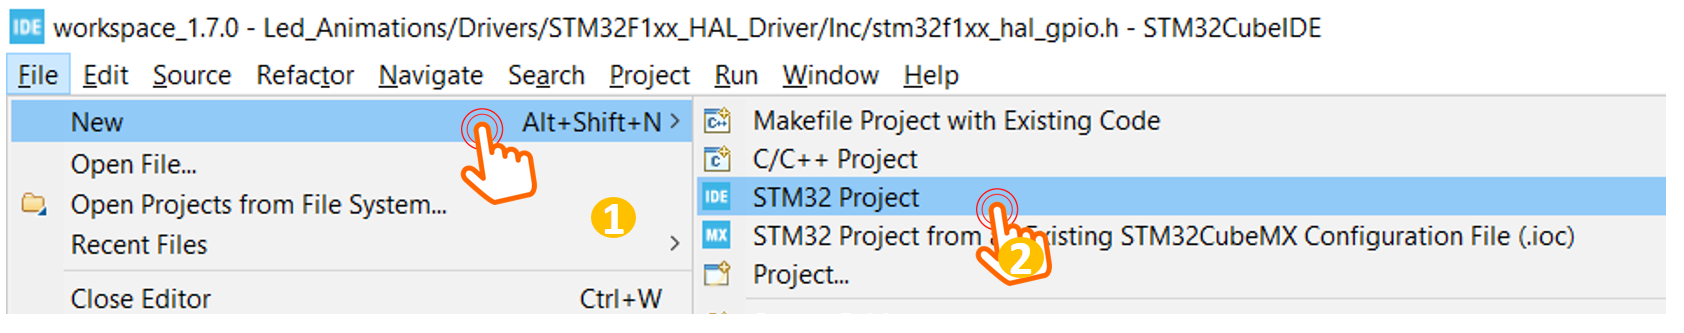
\includegraphics[width=5in]{source/picture/bai_1/stm_01.PNG}
    \caption{\textit{Create a new project on STM32CubeIDE}}
    \label{bai1_stm1}
\end{figure}

The IDE needs to download some packages, which normally takes time in this first time a project is created.\\

\textbf{Step 2: } Select the STM32F103C6 in the following dialog, then click on \textbf{Next}

\begin{figure}[!htp]
    \centering
    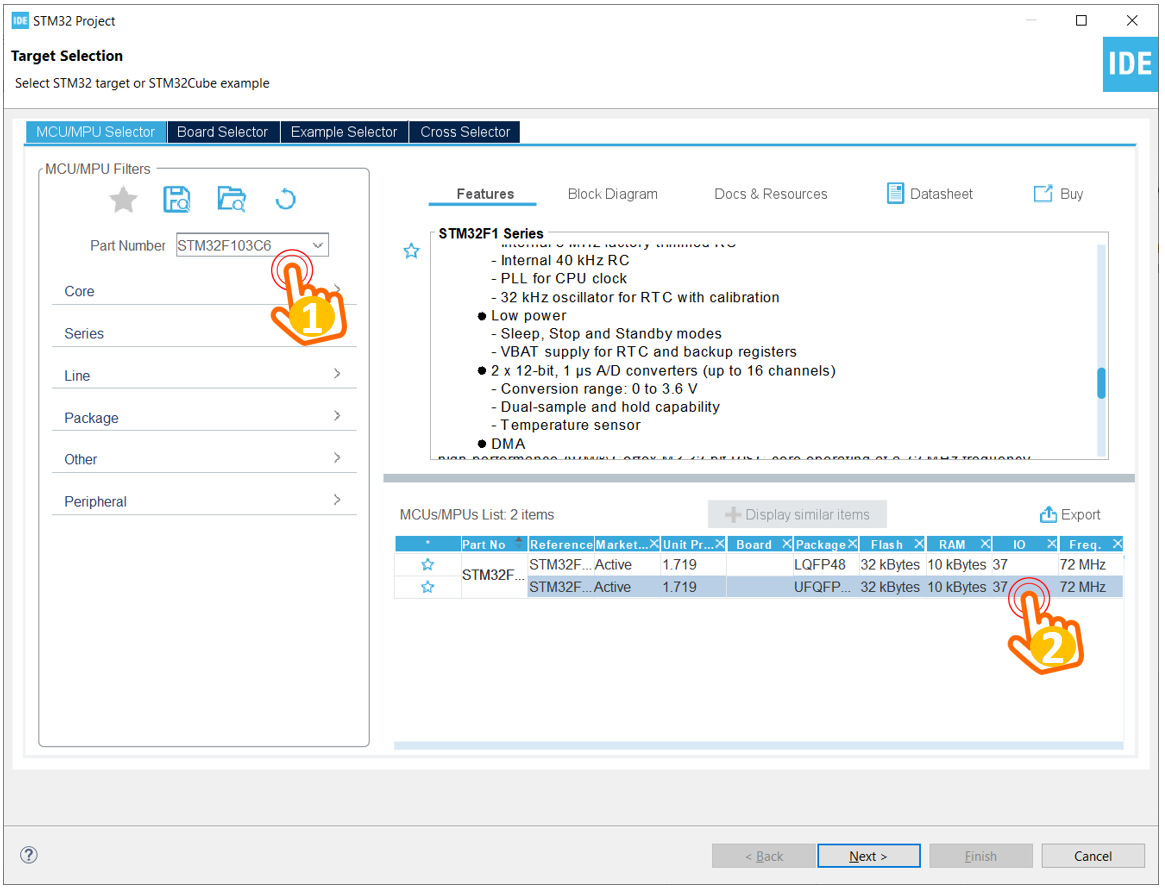
\includegraphics[width=5in]{source/picture/bai_1/stm_02.PNG}
    \caption{\textit{Select the target device}}
    \label{bai1_stm2}
\end{figure}

\textbf{Step 3: } Provide the \textbf{Name} and the \textbf{Location} for the project.

\newpage
\begin{figure}[!htp]
    \centering
    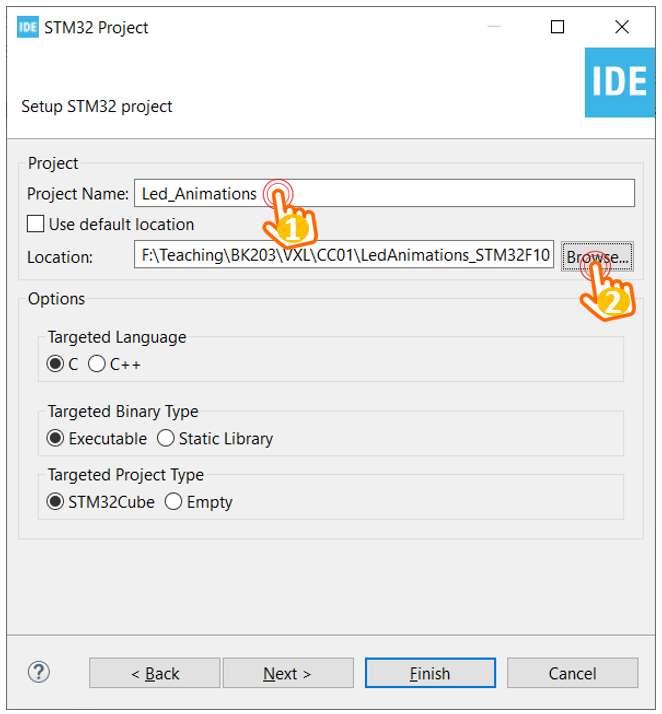
\includegraphics[width=3.5in]{source/picture/bai_1/stm_03.PNG}
    \caption{\textit{Select the target device}}
    \label{bai1_stm3}
\end{figure}

It is important to notice that the \textbf{Targeted Project Type} should be \textbf{STM32Cube}. In the case this option is disable, step 1 must be repeated. The location path should not contain special characters (e.g. the space). Finally, click on the \textbf{Next} button.\\

\textbf{Step 4: } On the last dialog, just keep the default firmware version and click on \textbf{Finish} button.

\begin{figure}[!htp]
    \centering
    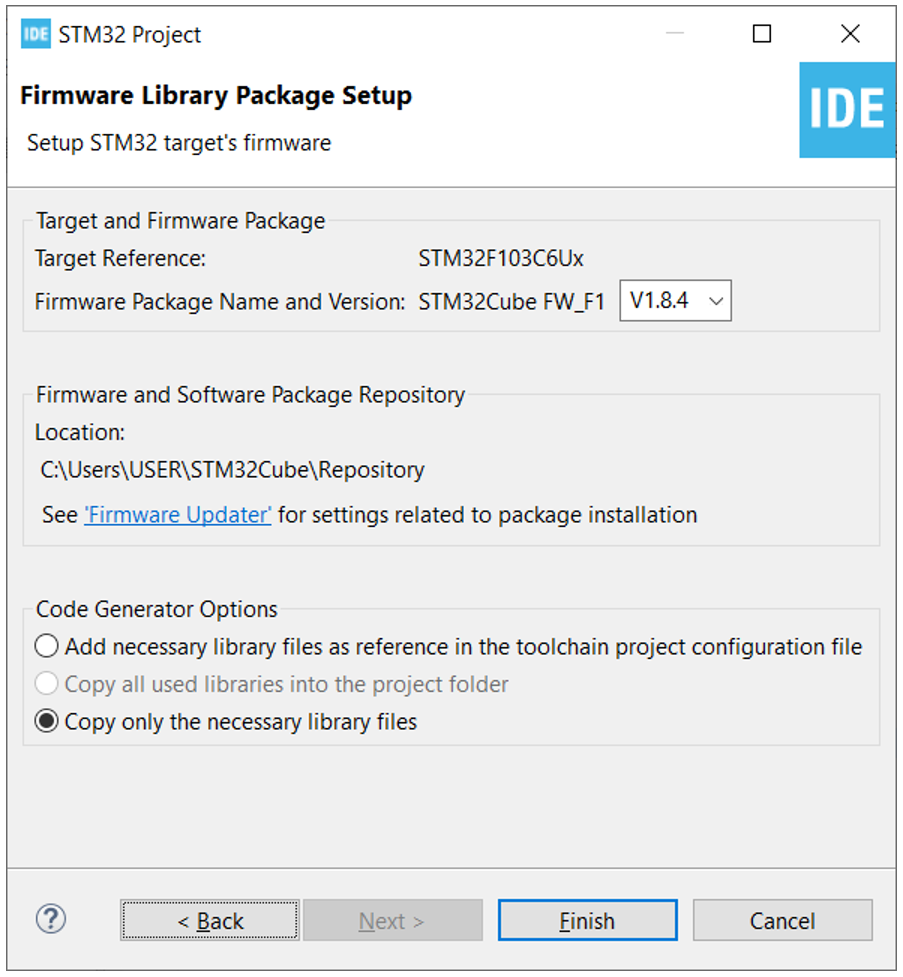
\includegraphics[width=3.5in]{source/picture/bai_1/stm_04.PNG}
    \caption{\textit{Keep default firmware version}}
    \label{bai1_stm4}
\end{figure}

\textbf{Step 5: } The project is created and the wizard for configuration is display. This utility from CubeIDE can simplify the configuration process for an ARM micro-controller like the STM32.

\begin{figure}[!htp]
    \centering
    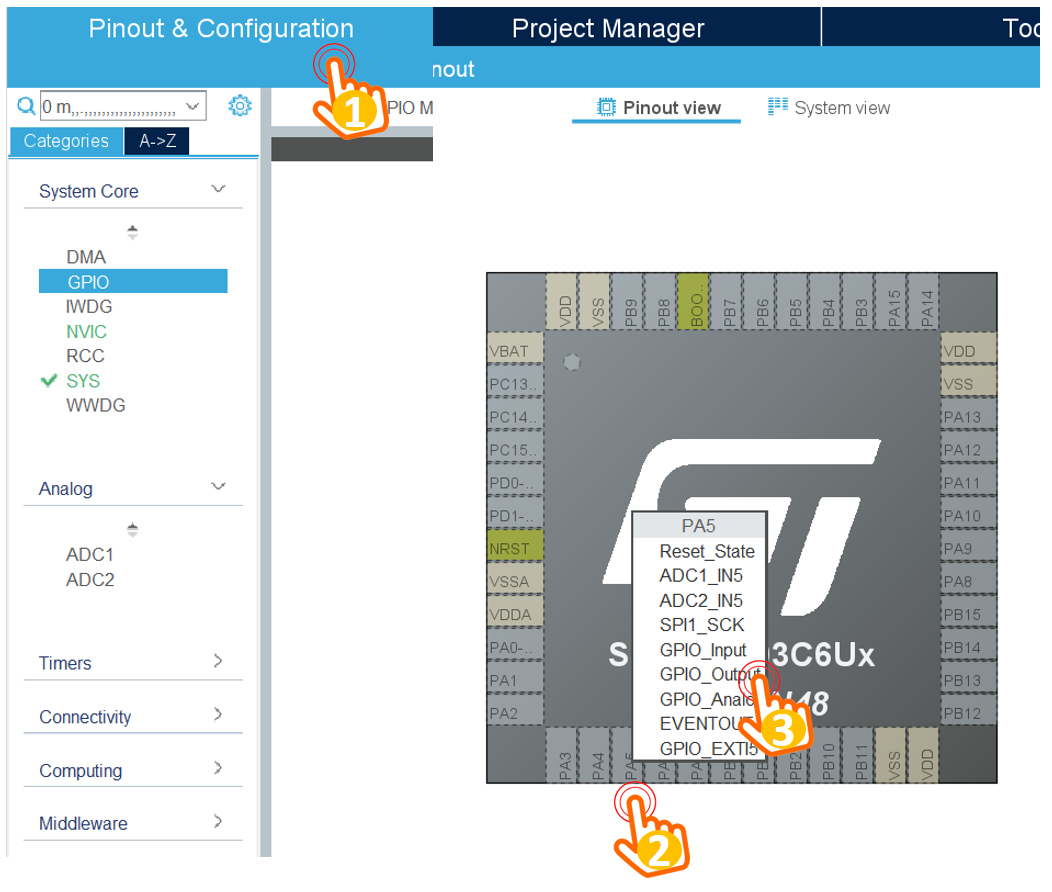
\includegraphics[width=3.5in]{source/picture/bai_1/stm_05.PNG}
    \caption{\textit{Set PA5 to GPIO Output mode}}
    \label{bai1_stm5}
\end{figure}

From the configuration windows, select \textbf{Pin configuration}, select the pin \textbf{PA5} and set to \textbf{GPIO Output} mode, since this pin is connected to an LED in the STM32 development kit.\\

\textbf{Step 6: } Right click on PA5 and select \textbf{Enter user lable}, and provide the name for this pin (e.g. \textbf{LED\_RED}). This step helps programming afterward more memorable.

\begin{figure}[!htp]
    \centering
    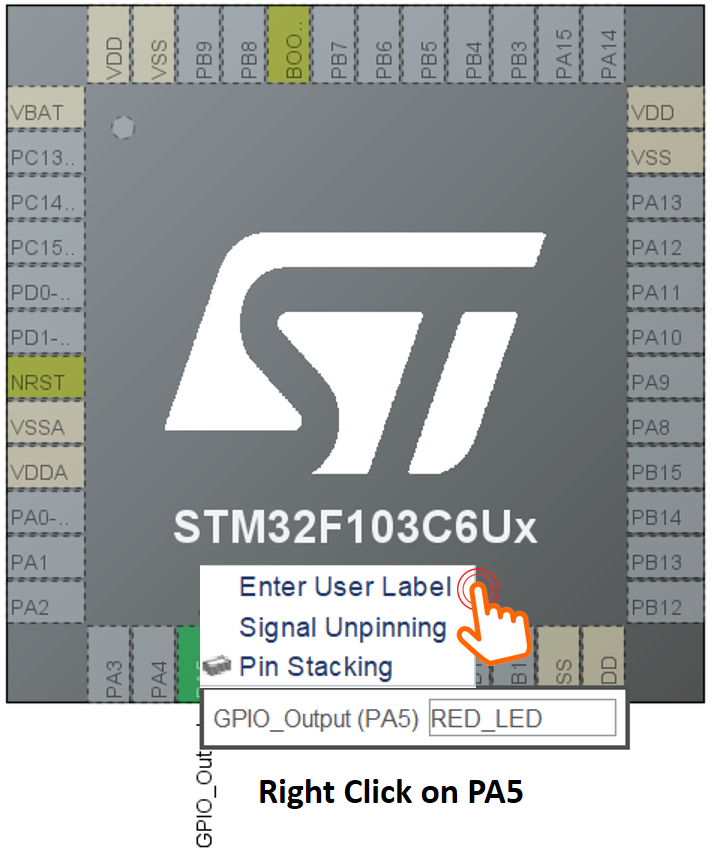
\includegraphics[width=2.5in]{source/picture/bai_1/stm_06.PNG}
    \caption{\textit{Provide a name for PA5}}
    \label{bai1_stm6}
\end{figure}

Finally, save the configuration process by pressing \textbf{Ctrl + S} and confirm this step by clicking on \textbf{OK} button. The code generation is started.\\

\textbf{Step 7: } Implement the first blinky project in the main function as follow:
\begin{lstlisting}[caption=First blinky LED project]
int main(void)
{
  /* USER CODE BEGIN 1 */

  /* USER CODE END 1 */

  /* MCU Configuration--------------------------------------------------------*/

  /* Reset of all peripherals, Initializes the Flash interface and the Systick. */
  HAL_Init();

  /* USER CODE BEGIN Init */

  /* USER CODE END Init */

  /* Configure the system clock */
  SystemClock_Config();

  /* USER CODE BEGIN SysInit */

  /* USER CODE END SysInit */

  /* Initialize all configured peripherals */
  MX_GPIO_Init();
  /* USER CODE BEGIN 2 */

  /* USER CODE END 2 */

  /* Infinite loop */
  /* USER CODE BEGIN WHILE */
 
  while (1)
  {
	  HAL_GPIO_TogglePin(LED_RED_GPIO_Port, LED_RED_Pin);
	  HAL_Delay(1000);
    /* USER CODE END WHILE */

    /* USER CODE BEGIN 3 */
  }
  /* USER CODE END 3 */
}
\end{lstlisting}

Actually, what is added to the main function is line number 34 and 35. Please put your code in a right place, otherwise it can be deleted when the code is generated (e.g. change the configuration of the project). When coding, frequently use the suggestions by pressing \textbf{Ctrl+Space}.

\textbf{Step 7: } Due to the simulation on Proteus, the hex file should be generated from STM32Cube IDE. From menu \textbf{Project}, select \textbf{Properties} to open the dialog bellow:

\begin{figure}[!htp]
    \centering
    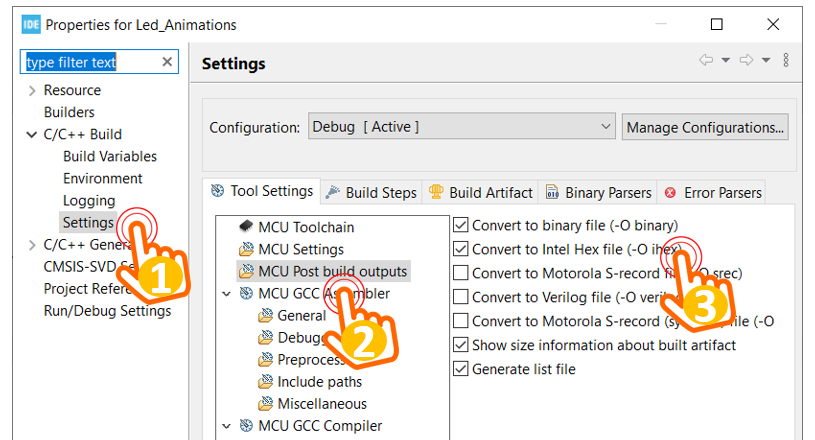
\includegraphics[width=5in]{source/picture/bai_1/stm_07.PNG}
    \caption{\textit{Config for hex file output}}
    \label{bai1_pic5}
\end{figure}

Navigate to \textbf{C/C++ Build}, select \textbf{Settings, MCU Post build outputs}, and check to the \textbf{Intel Hex file}. \\

\textbf{Step 8: } Build the project by clicking on menu \textbf{Project} and select \textbf{Build Project}. Please check on the output console of the IDE to be sure that the hex file is generated, as follow:

\begin{figure}[!htp]
    \centering
    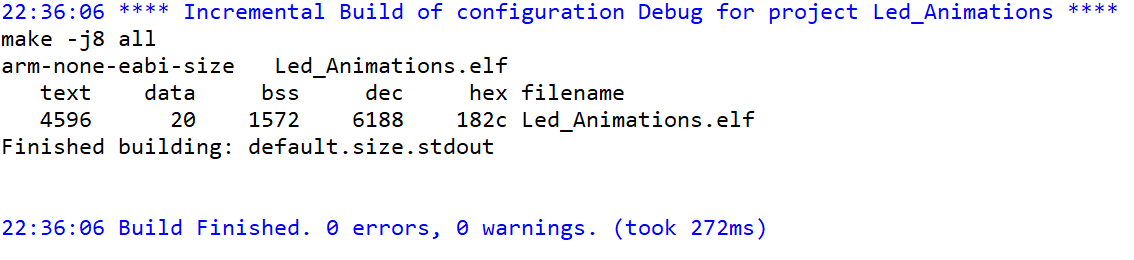
\includegraphics[width=5in]{source/picture/bai_1/stm_08.PNG}
    \caption{\textit{Compile the project and generate Hex file}}
    \label{bai1_pic8}
\end{figure}

The hex file is located under the \textbf{Debug} folder of your project, which is used for the simulation in Proteus afterward. In the case a development kit is connected to your PC, from menu \textbf{Run}, select \textbf{Run} to download the program to the hardware platform. \\

In the case there are multiple project in a work-space, double click on the project name to activate this project. Whenever a project is built, check the output files to make sure that you are working in a right project.


\newpage
\subsection{Simulation on Proteus}
For an online training, a simulation on Proteus can be used. The details to create an STM32 project on Proteus are described bellow.\\

\textbf{Step 1: } Launch Proteus (\textbf{with administration access}) and from menu \textbf{File}, select \textbf{New Project}.\\

\begin{figure}[!htp]
    \centering
    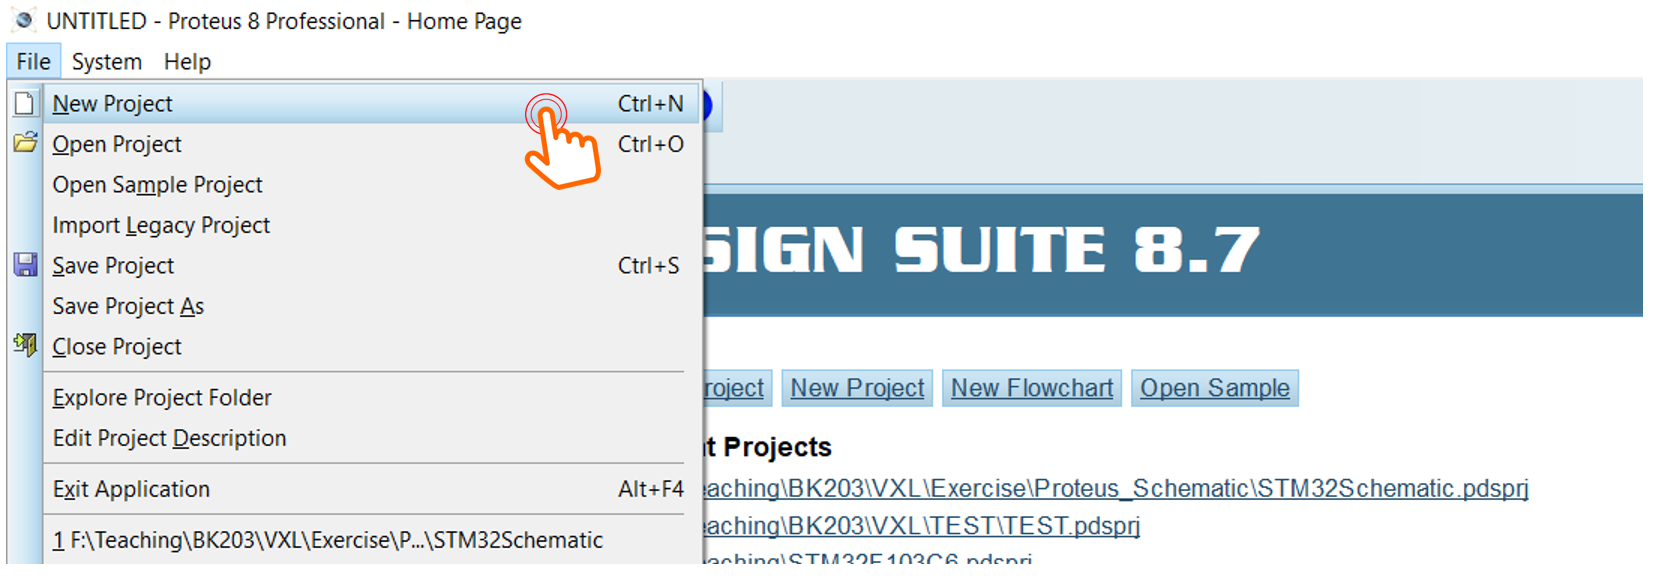
\includegraphics[width=5in]{source/picture/bai_1/pic5.PNG}
    \caption{\textit{Create a new project on Proteus}}
    \label{bai1_pic5}
\end{figure}


\textbf{Step 2: } Provide the name and the location of the project, then click on \textbf{Next} button.\\

\begin{figure}[!htp]
    \centering
    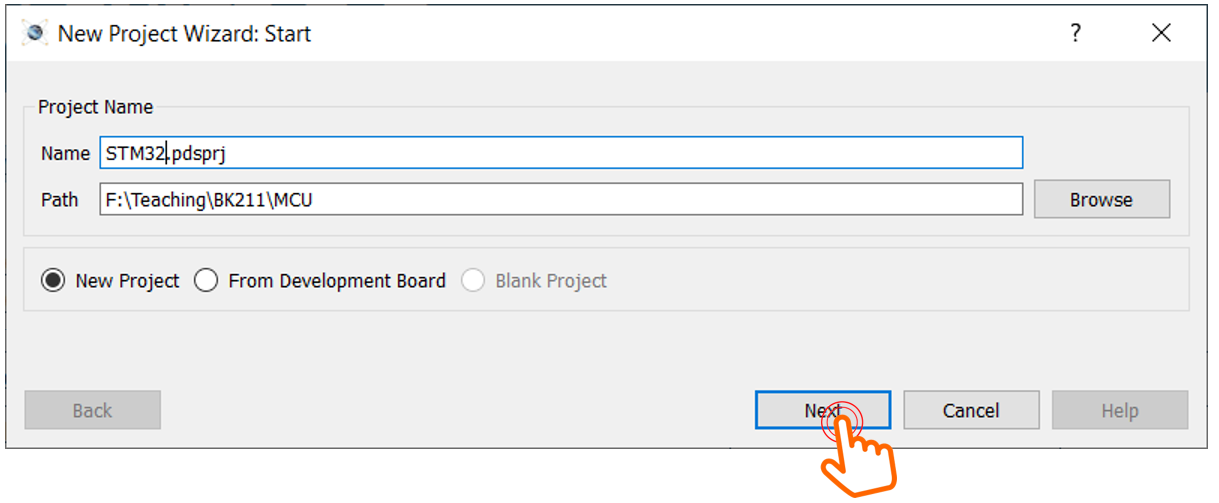
\includegraphics[width=4in]{source/picture/bai_1/pic6.PNG}
    \caption{\textit{Provide project name and location}}
    \label{bai1_pic6}
\end{figure}

\textbf{Step 3: } For following dialog, just click on \textbf{Next} button as just a schematic is required for the lab.

\begin{figure}[!htp]
    \centering
    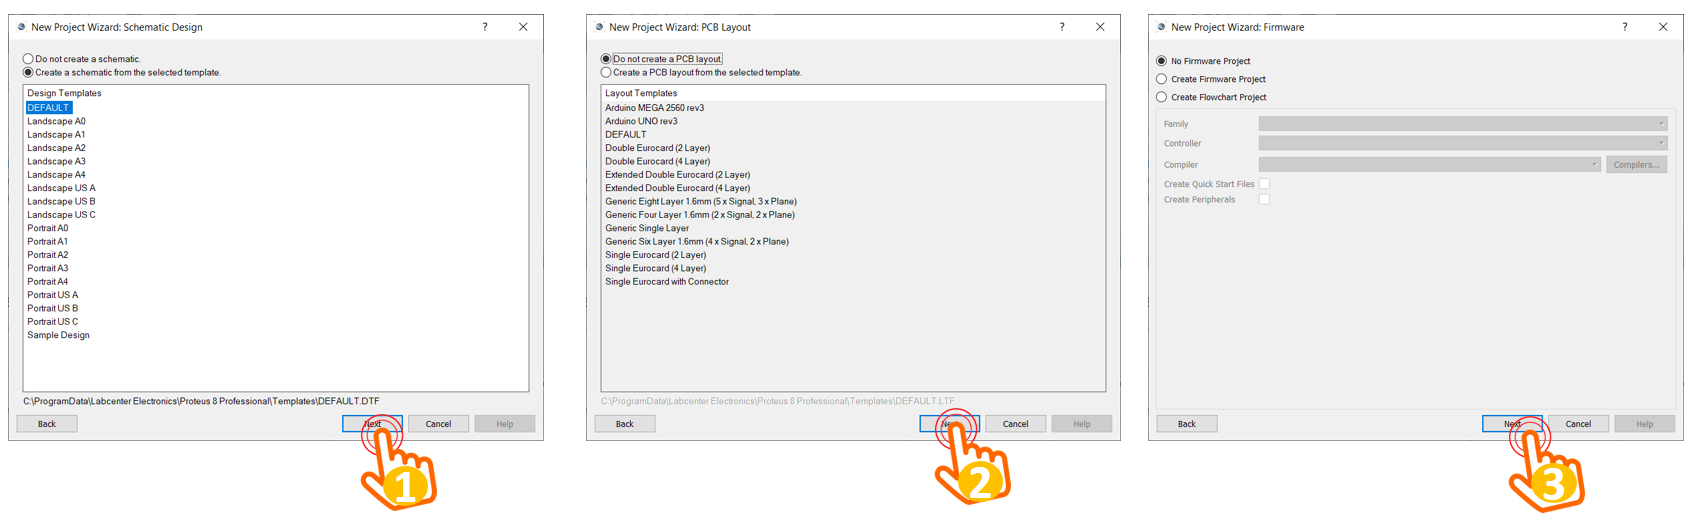
\includegraphics[width=5.5in]{source/picture/bai_1/pic7.PNG}
    \caption{\textit{Keep the default options by clicking on Next}}
    \label{bai1_pic7}
\end{figure}
\newpage
\textbf{Step 4: } Finally, click on \textbf{Finish} button to close the project wizard. \\

\begin{figure}[!htp]
    \centering
    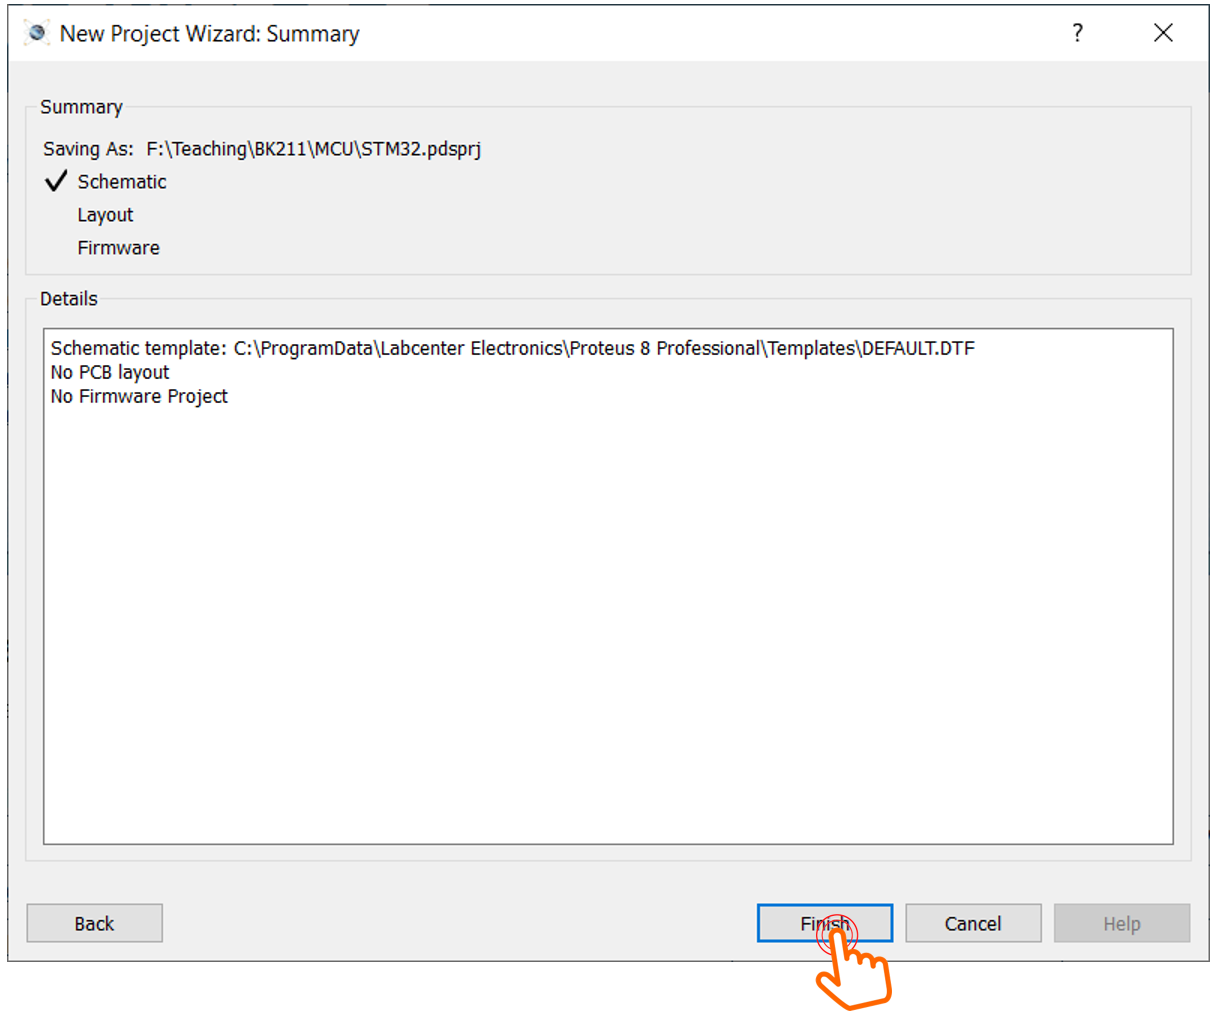
\includegraphics[width=4in]{source/picture/bai_1/pic8.PNG}
    \caption{\textit{Finish the project wizard}}
    \label{bai1_pic8}
\end{figure}

\textbf{Step 5: } On the main page of the project, right click to select \textbf{Place, Components, From Libraries}, as follows:
\begin{figure}[!htp]
    \centering
    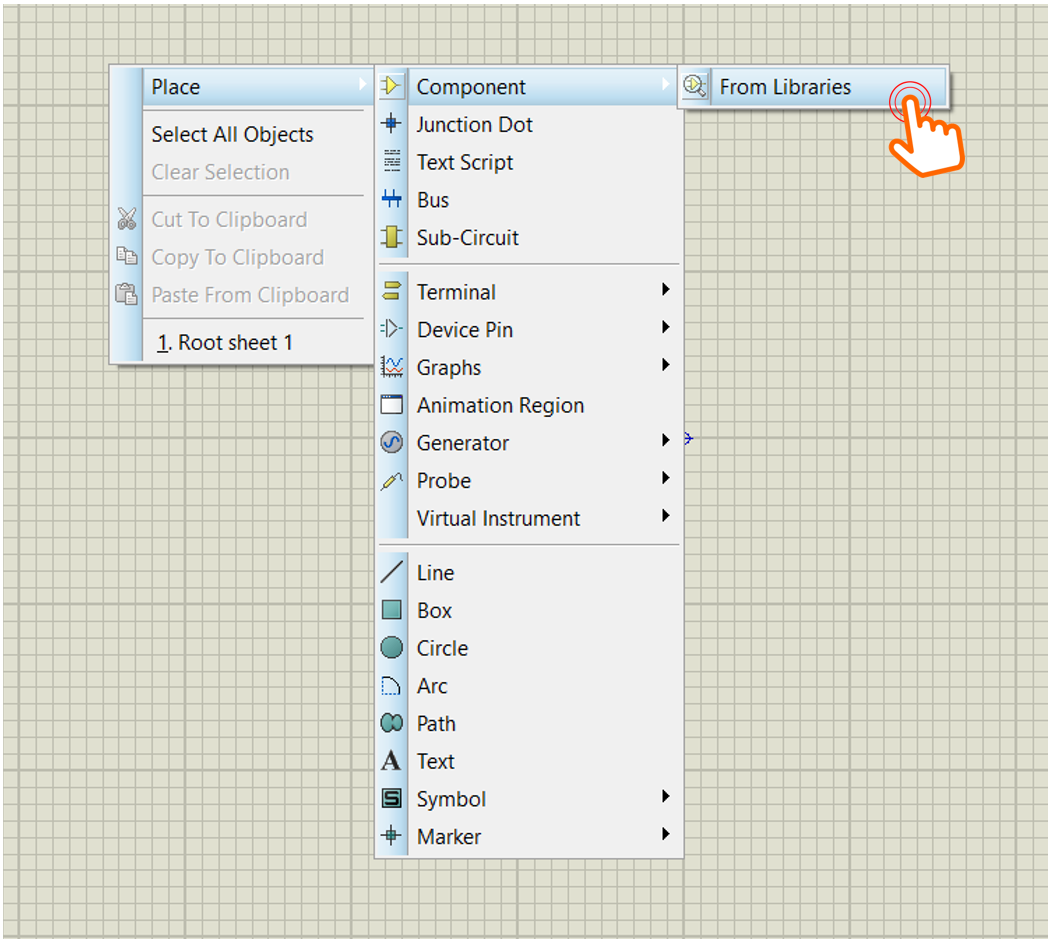
\includegraphics[width=4in]{source/picture/bai_1/pic9.PNG}
    \caption{\textit{Select a component from the library}}
    \label{bai1_pic9}
\end{figure}

\textbf{If there is an error with no library found, please restart the Proteus software with Run as administrator option.\\}

\textbf{Step 6: } From the list of components in the library, select STM32F103C6, as follows:

\begin{figure}[!htp]
    \centering
    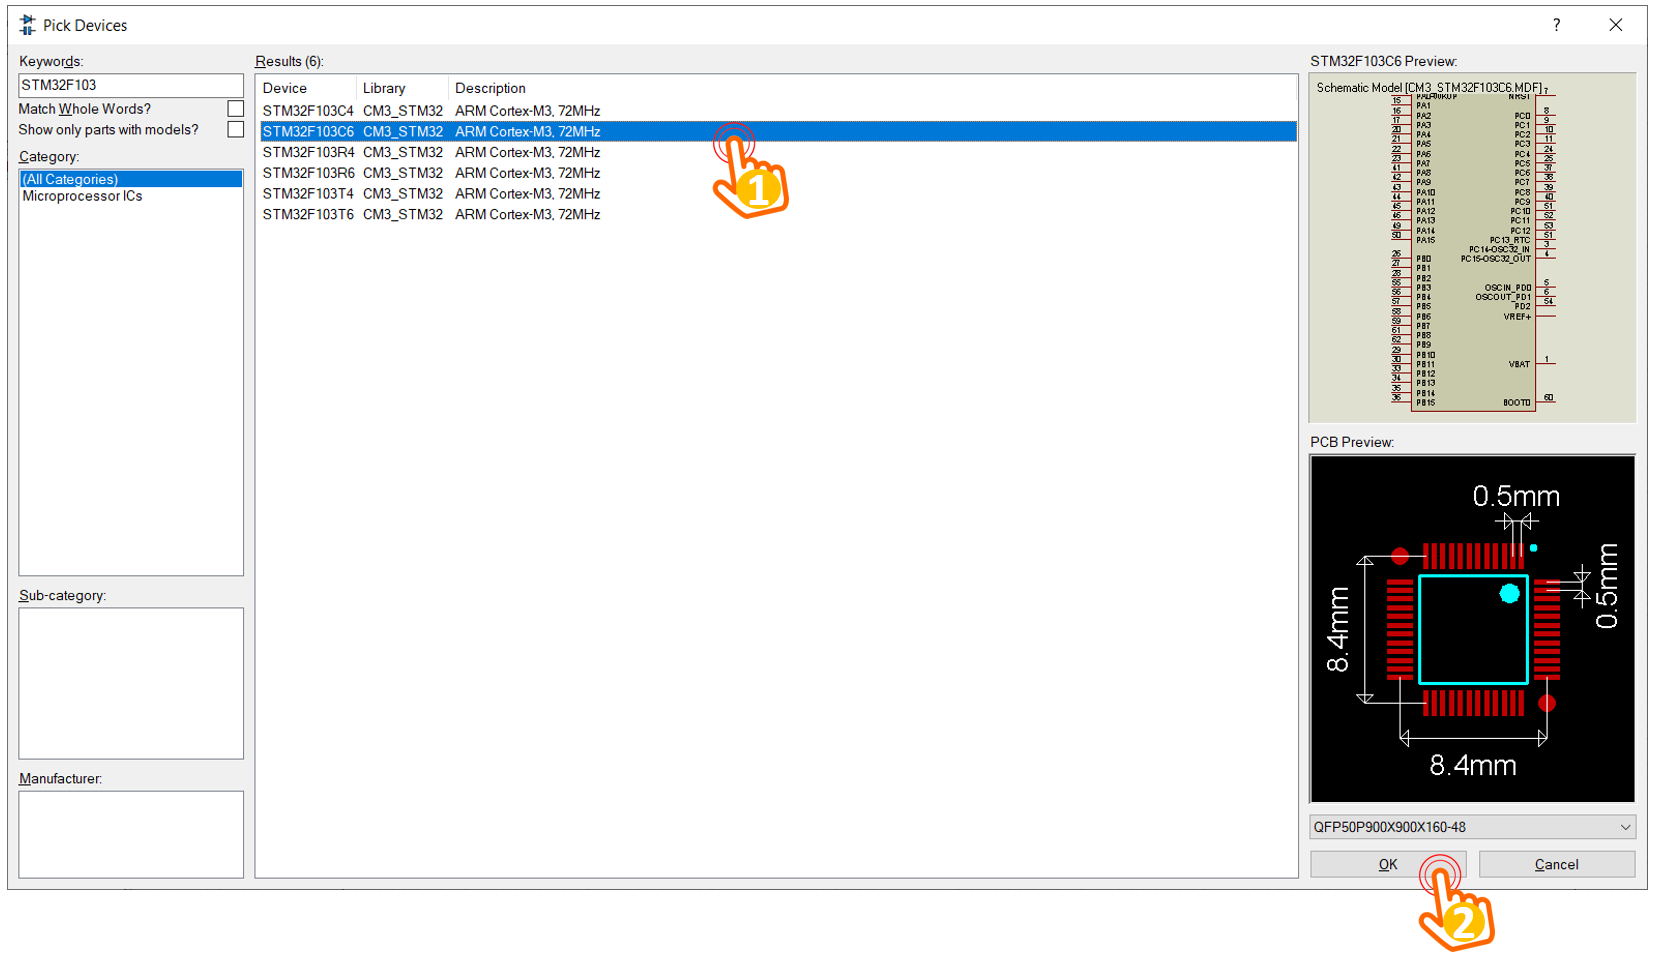
\includegraphics[width=5.5in]{source/picture/bai_1/pic10.PNG}
    \caption{\textit{Select STM32F103C6}}
    \label{bai1_pic10}
\end{figure}

Repeat step 5 and 6 to select an LED, named \textbf{LED-RED} in Proteus. Finally, these components are appeared on the DEVICES windows, which is on left hand side as follows:
\begin{figure}[!htp]
    \centering
    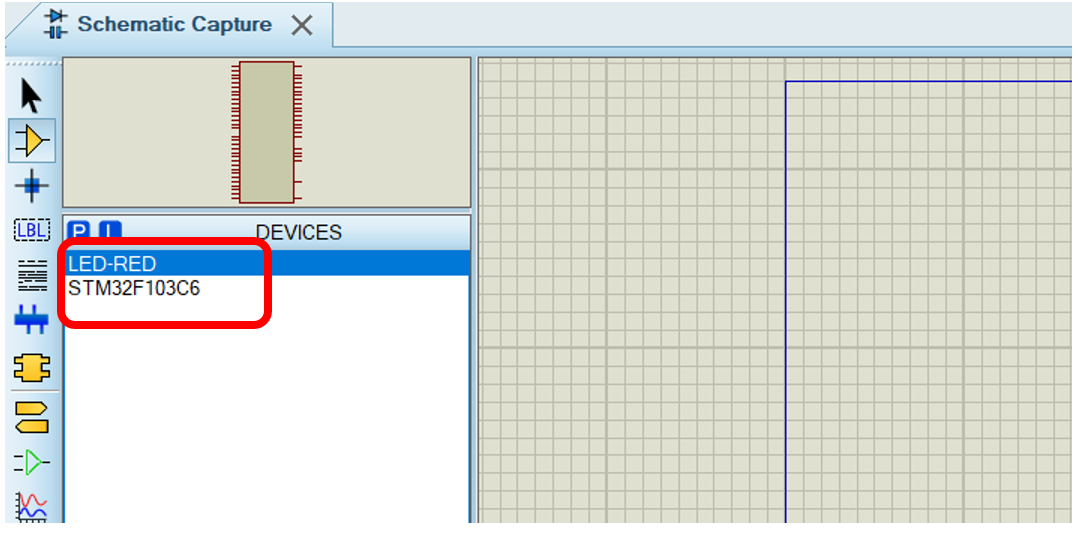
\includegraphics[width=4in]{source/picture/bai_1/pic11.PNG}
    \caption{\textit{STM32 and an LED in the project}}
    \label{bai1_pic9}
\end{figure}

\textbf{Step 7: } Place the components to the project: right click on the main page, select on \textbf{Place, Component}, and select device added in Step 6. To add the Power and the Ground,  right click on the main page, select on \textbf{Place, Terminal}. The result in this step is expected as follows:
\newpage
\begin{figure}[!htp]
    \centering
    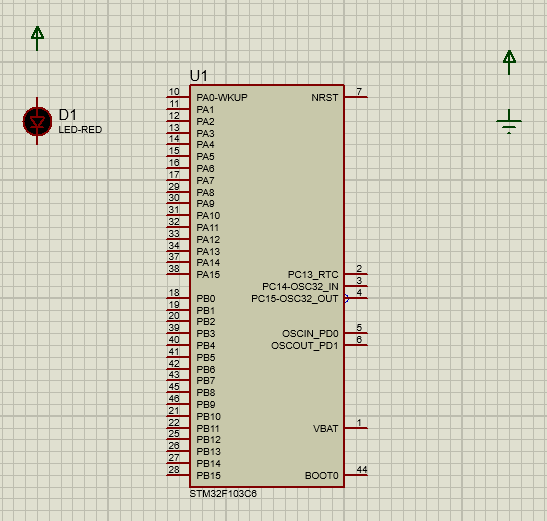
\includegraphics[width=4in]{source/picture/bai_1/pic14.PNG}
    \caption{\textit{Place components to the project}}
    \label{bai1_pic14}
\end{figure}

\textbf{Step 8: } Start wiring the circuit. The negative pin of the LED is connected to PA5 while its positive pin is connected to the power supply. For the power and the ground on the right, just make a short wire, which will labeled in the next step.

\begin{figure}[!htp]
    \centering
    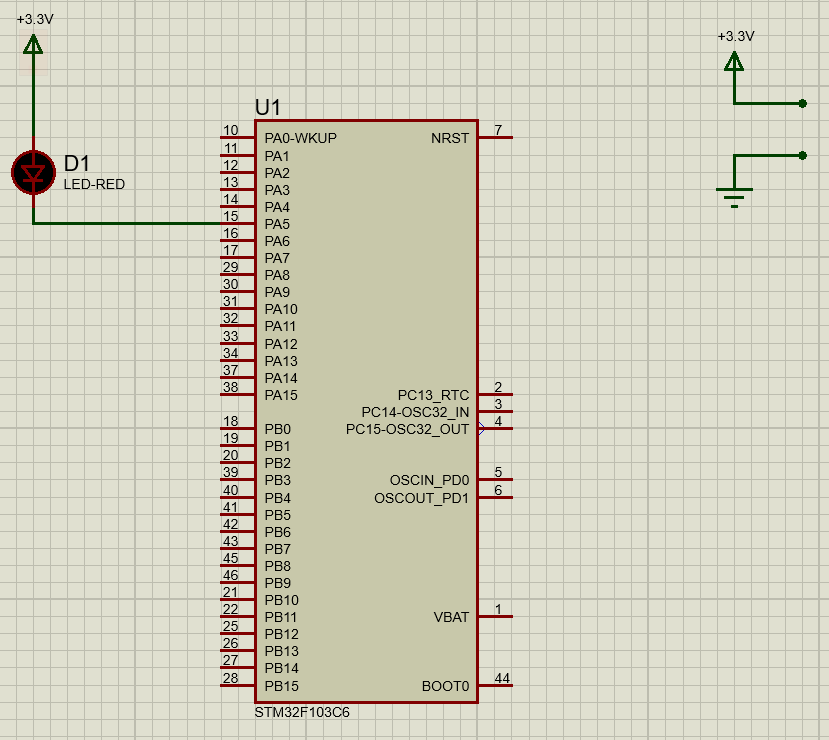
\includegraphics[width=4in]{source/picture/bai_1/pic15.PNG}
    \caption{\textit{Connect components and set the power to 3.3V}}
    \label{bai1_pic15}
\end{figure}

In this step, also double click on the power supply in order to provide the String property to \textbf{+3.3V}.

\textbf{Step 8: } Right click on the wire of the power supply and the ground, and select \textbf{Place wire Label}

\begin{figure}[!htp]
    \centering
    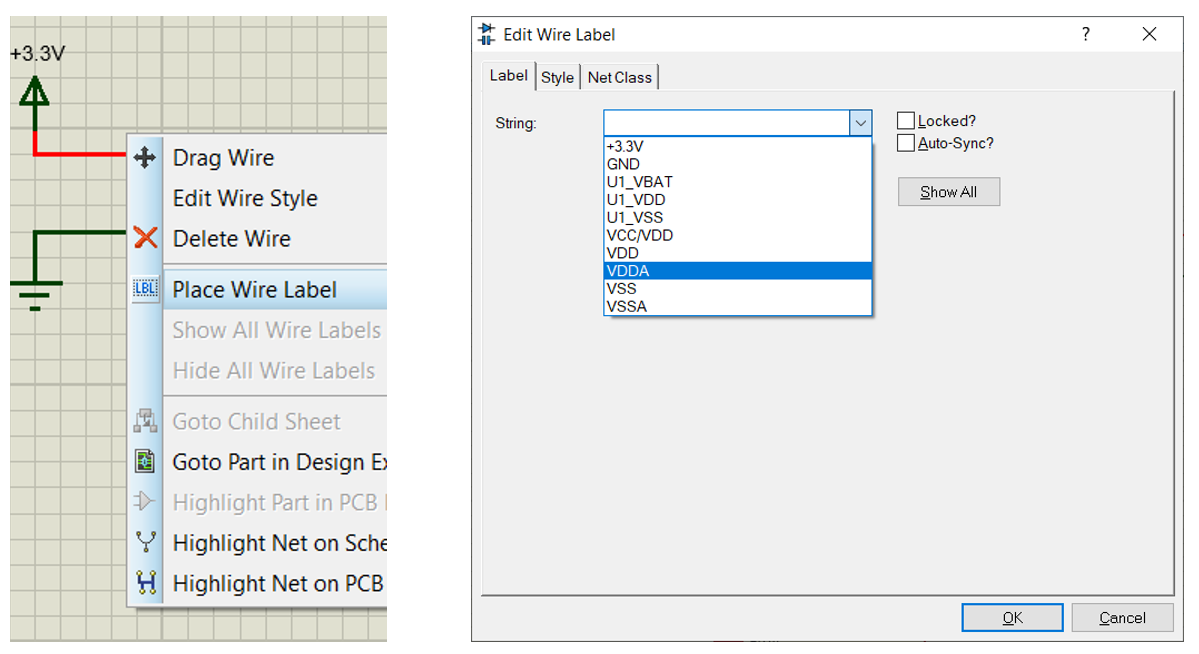
\includegraphics[width=4in]{source/picture/bai_1/pic16.PNG}
    \caption{\textit{Place label for Power and Ground}}
    \label{bai1_pic16}
\end{figure}

This step is required as VDDA and VSSA of the STM32 must be connected to provide the reference voltage. Therefore, VDDA is connected to 3.3V, while the VSSA is connected to the Ground. Finally, the image of our schematic is shown bellow:

\begin{figure}[!htp]
    \centering
    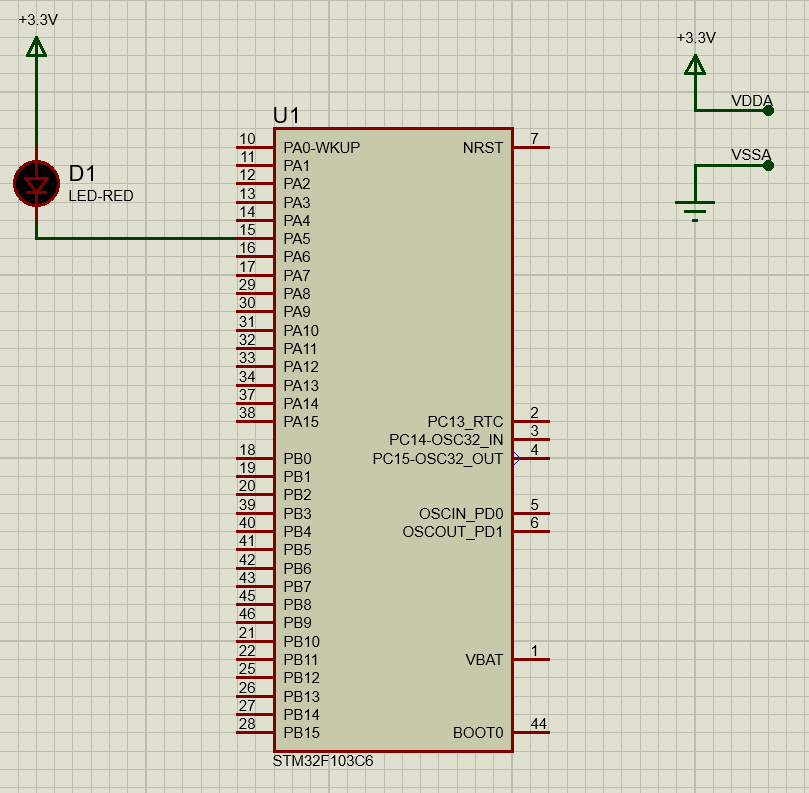
\includegraphics[width=4in]{source/picture/bai_1/pic17.PNG}
    \caption{\textit{Finalize the schematic}}
    \label{bai1_pic17}
\end{figure}
\newpage
\textbf{Step 9: } Double click on the STM32, and set the \textbf{Program File} to the Hex file, which is generated from Cube IDE, as following:

\begin{figure}[!htp]
    \centering
    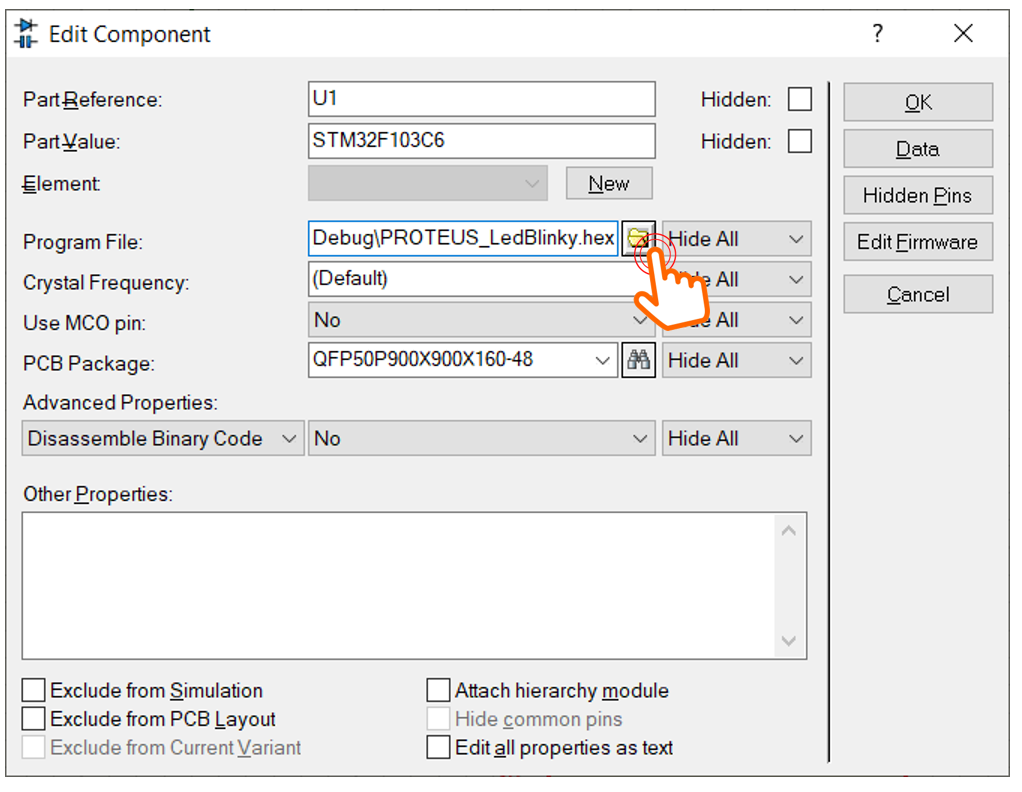
\includegraphics[width=4in]{source/picture/bai_1/pic18.PNG}
    \caption{\textit{Set the program of the STM32 to the hex file from Cube IDE}}
    \label{bai1_pic18}
\end{figure}

From now, the simulation is ready to start by clicking on the menu \textbf{Debug}, and select on \textbf{Run simulation}. To stop the simulation, click on \textbf{Debug} and select \textbf{Stop VMS Debugging}. Moreover, there are some quick access bottom on the left corner of the Proteus to start or stop the simulation, as shown following:\\
\begin{figure}[!htp]
    \centering
    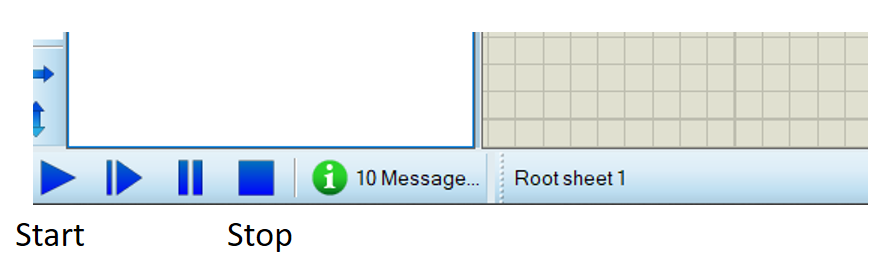
\includegraphics[width=4in]{source/picture/bai_1/pic18a.PNG}
    \caption{\textit{Quick access buttons to start and stop the simulation}}
    \label{bai1_pic18}
\end{figure}

If everything is success, students can see the LED is blinking every second. Please stop the simulation before updating the project, either in Proteus or STM32Cube IDE. However, the step 9 (set the program file for STM32 in Proteus) is required to do once. Beside the toggle instruction, student can set or reset a pin as following:

\begin{lstlisting}[caption=An example for LED blinky]
while (1){
  HAL_GPIO_WritePin(LED_RED_GPIO_Port, LED_RED_Pin, GPIO_PIN_SET);
  HAL_Delay(1000);
  HAL_GPIO_WritePin(LED_RED_GPIO_Port, LED_RED_Pin, GPIO_PIN_RESET);
  HAL_Delay(1000);
}
\end{lstlisting}
\newpage
\subsection{Exercise and Report}
\subsubsection{Exercise 1}
From the simulation on Proteus, one more LED is connected to pin \textbf{PA6} of the STM32 (negative pin of the LED is connected to PA6). The component suggested in this exercise is \textbf{LED-YELLOW}, which can be found from the device list.\\



In this exercise, the status of two LEDs are switched every 2 seconds, as demonstrated in the figure bellow.

\begin{figure}[!htp]
    \centering
    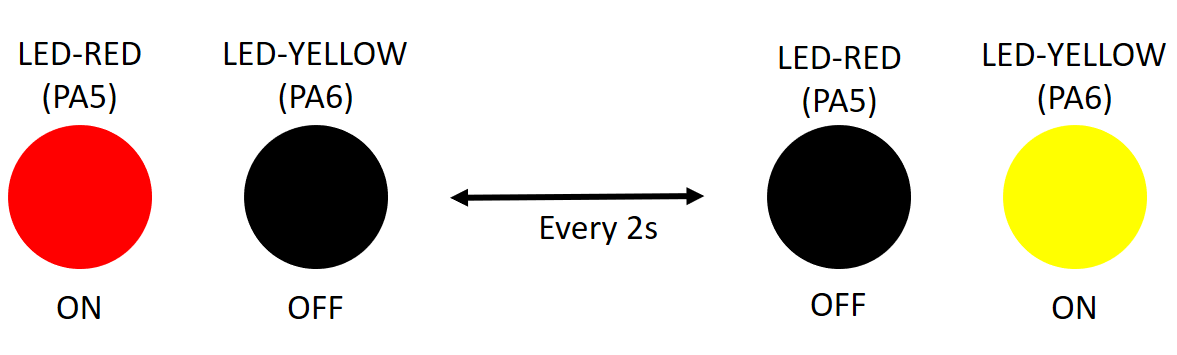
\includegraphics[width=5in]{source/picture/bai_1/pic1.PNG}
    \caption{\textit{State transitions for 2 LEDs}}
    \label{bai1_pic1}
\end{figure}

\textbf{Report 1: } The Proteus schematic contains two LEDs connected to GPIO output pins of the STM32. In this implementation, the red LED is connected to \textbf{PA5} and the yellow LED is connected to \textbf{PA6}. Both LEDs are connected in active-low mode: the positive terminal of each LED is connected to the 3.3V supply through a current-limiting resistor, while the negative terminal is connected to the GPIO pin. Therefore, writing logic 0 to the GPIO pin turns the LED on, and writing logic 1 turns the LED off.\\

\begin{figure}[!htp]
    \centering
    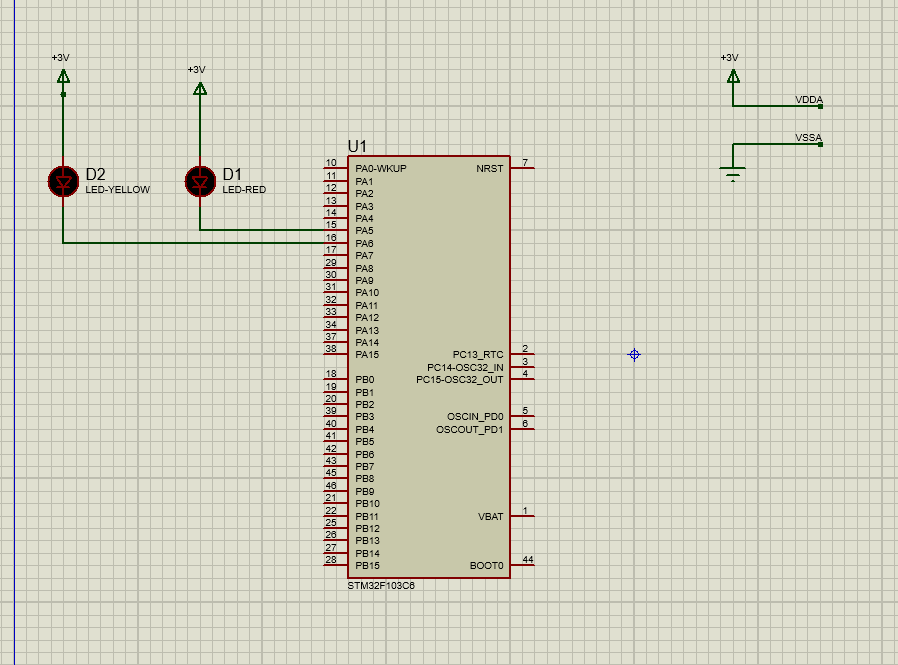
\includegraphics[width=5in]{source/picture/bai_1/lab1_ex1.png}
    \caption{\href{https://raw.githubusercontent.com/quangnguyencomeng/CO3009-261-CC-2453052/main/Lab/LAB01/PROTEUS/LED_BLINKY.pdsprj}{\textit{Proteus schematic for Exercise 1 (download project)}}}
    \label{bai1_ex1_schematic}
\end{figure}

The demonstration video for this exercise is available at:
\begin{center}
    \url{https://github.com/quangnguyencomeng/CO3009-261-CC-2453052/blob/main/Lab/lab_reports/source/vids/lab1_ex1.mp4}
\end{center}

\textbf{Report 2: } The source code inside the infinite loop is shown below. The program turns on the red LED while turning off the yellow LED for 2 seconds, then switches the states of the two LEDs for another 2 seconds.

\begin{lstlisting}[caption=Source code for Exercise 1]
while (1)
{
  /* USER CODE END WHILE */

  // RED: PA5, active-low
  // YELLOW: PA6, active-low
  // Phase 1: red ON, yellow OFF
  HAL_GPIO_WritePin(LED_RED_GPIO_Port, LED_RED_Pin, GPIO_PIN_RESET);
  HAL_GPIO_WritePin(LED_YELLOW_GPIO_Port, LED_YELLOW_Pin, GPIO_PIN_SET);
  HAL_Delay(2000);

  // Phase 2: red OFF, yellow ON
  HAL_GPIO_WritePin(LED_RED_GPIO_Port, LED_RED_Pin, GPIO_PIN_SET);
  HAL_GPIO_WritePin(LED_YELLOW_GPIO_Port, LED_YELLOW_Pin, GPIO_PIN_RESET);
  HAL_Delay(2000);

  /* USER CODE BEGIN 3 */
}
\end{lstlisting}

\subsubsection{Exercise 2}
Extend the first exercise to simulate the behavior of a traffic light. A third LED, named \textbf{LED-GREEN} is added to the system, which is connected to \textbf{PA7}. A cycle in this traffic light is 5 seconds for the RED, 2 seconds for the YELLOW and 3 seconds for the GREEN. The LED-GREEN is also controlled by its negative pin.\\

Similarly, the report in this exercise includes the schematic of your circuit and a your source code in the while loop.

\textbf{Report 1: } The Proteus schematic is extended from Exercise 1 by adding one more LED for the green signal. In this traffic-light circuit, the red LED is connected to \textbf{PA5}, the yellow LED is connected to \textbf{PA6}, and the green LED is connected to \textbf{PA7}. These three pins are configured as GPIO outputs. The LEDs are still connected in active-low mode, so a GPIO output value of \texttt{GPIO\_PIN\_RESET} turns the selected LED on, while \texttt{GPIO\_PIN\_SET} turns it off.

\begin{figure}[!htp]
    \centering
    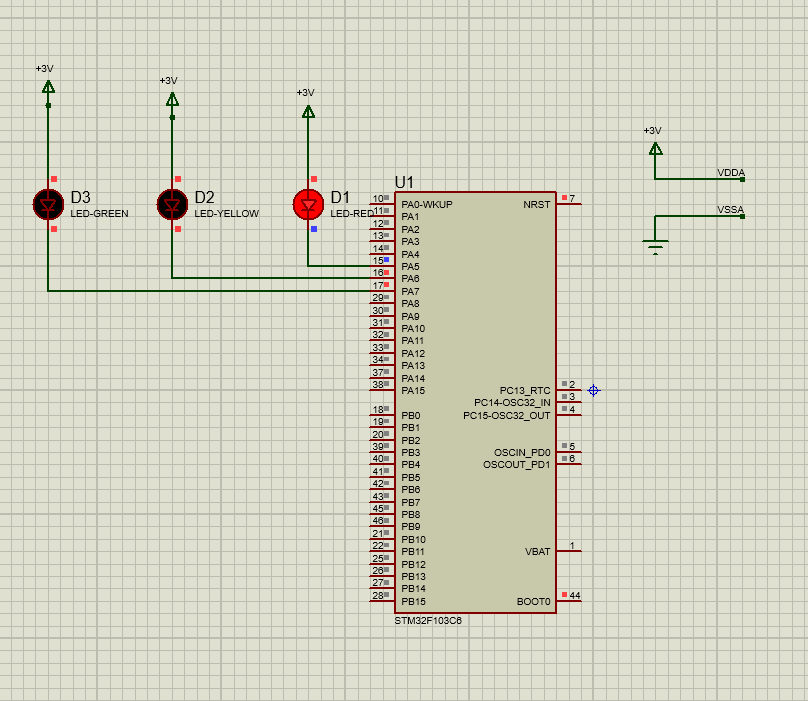
\includegraphics[width=5in]{source/picture/bai_1/lab1_ex2.png}
    \caption{\textit{Proteus schematic for Exercise 2}}
    \label{bai1_ex2_schematic}
\end{figure}

The demonstration video for this exercise is available at:
\begin{center}
    \url{https://github.com/quangnguyencomeng/CO3009-261-CC-2453052/blob/main/Lab/lab_reports/source/vids/lab1_ex2.mp4}
\end{center}

\textbf{Report 2: } The source code inside the infinite loop is shown below. The program turns on the red LED for 5 seconds, then turns on the green LED for 3 seconds, and finally turns on the yellow LED for 2 seconds. Since the LEDs are active-low, the active LED is written with \texttt{GPIO\_PIN\_RESET} and the inactive LEDs are written with \texttt{GPIO\_PIN\_SET}.

\begin{lstlisting}[caption=Source code for Exercise 2]
while (1)
{
  /* USER CODE END WHILE */

  // Phase 1: red ON, yellow OFF, green OFF
  HAL_GPIO_WritePin(LED_RED_GPIO_Port, LED_RED_Pin, GPIO_PIN_RESET);
  HAL_GPIO_WritePin(LED_YELLOW_GPIO_Port, LED_YELLOW_Pin, GPIO_PIN_SET);
  HAL_GPIO_WritePin(LED_GREEN_GPIO_Port, LED_GREEN_Pin, GPIO_PIN_SET);
  HAL_Delay(5000);

  // Phase 2: red OFF, yellow OFF, green ON
  HAL_GPIO_WritePin(LED_RED_GPIO_Port, LED_RED_Pin, GPIO_PIN_SET);
  HAL_GPIO_WritePin(LED_YELLOW_GPIO_Port, LED_YELLOW_Pin, GPIO_PIN_SET);
  HAL_GPIO_WritePin(LED_GREEN_GPIO_Port, LED_GREEN_Pin, GPIO_PIN_RESET);
  HAL_Delay(3000);

  // Phase 3: red OFF, yellow ON, green OFF
  HAL_GPIO_WritePin(LED_RED_GPIO_Port, LED_RED_Pin, GPIO_PIN_SET);
  HAL_GPIO_WritePin(LED_YELLOW_GPIO_Port, LED_YELLOW_Pin, GPIO_PIN_RESET);
  HAL_GPIO_WritePin(LED_GREEN_GPIO_Port, LED_GREEN_Pin, GPIO_PIN_SET);
  HAL_Delay(2000);

  /* USER CODE BEGIN 3 */
}
\end{lstlisting}

\subsubsection{Exercise 3}
Extend to the 4-way traffic light. Arrange 12 LEDs in a nice shape to simulate the behaviors of a traffic light. A reference design can be found in the figure bellow.

\begin{figure}[!htp]
    \centering
    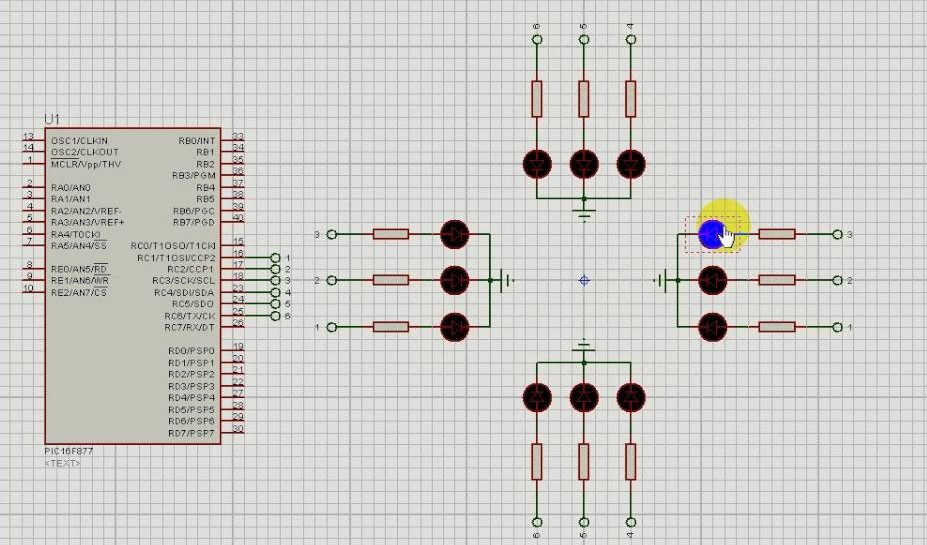
\includegraphics[width=5in]{source/picture/bai_1/pic2.jpg}
    \caption{\textit{Reference design for a 4 way traffic light}}
    \label{bai1_pic2}
\end{figure}

\textbf{Report 1: } The Proteus simulation uses two traffic-light directions: left-right and up-down. Each direction has three LEDs: red, yellow, and green. The two screenshots below show two important states of the traffic-light cycle. In the first state, the left-right direction is green while the up-down direction is red. In the next transition state, the left-right direction changes to yellow while the up-down direction remains red.

\begin{figure}[!htp]
    \centering
    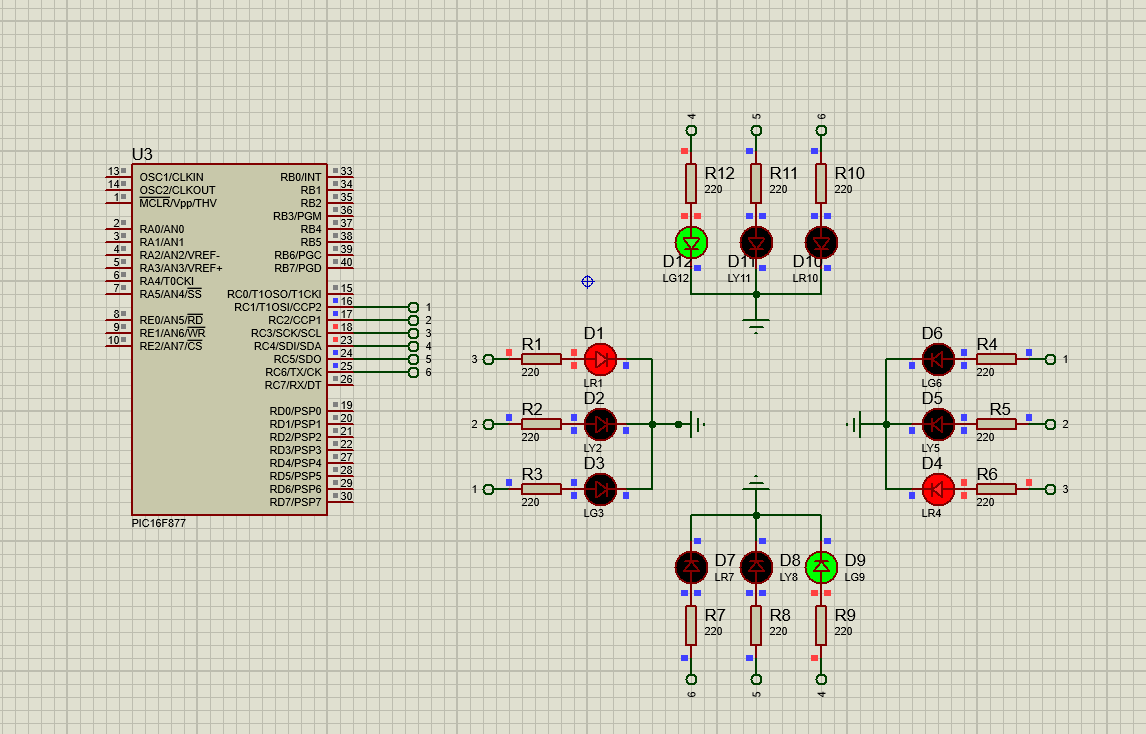
\includegraphics[width=5in]{source/picture/bai_1/lab1_ex3.1.png}
    \caption{\textit{Exercise 3 simulation: left-right green and up-down red}}
    \label{bai1_ex3_state_green_red}
\end{figure}

\begin{figure}[!htp]
    \centering
    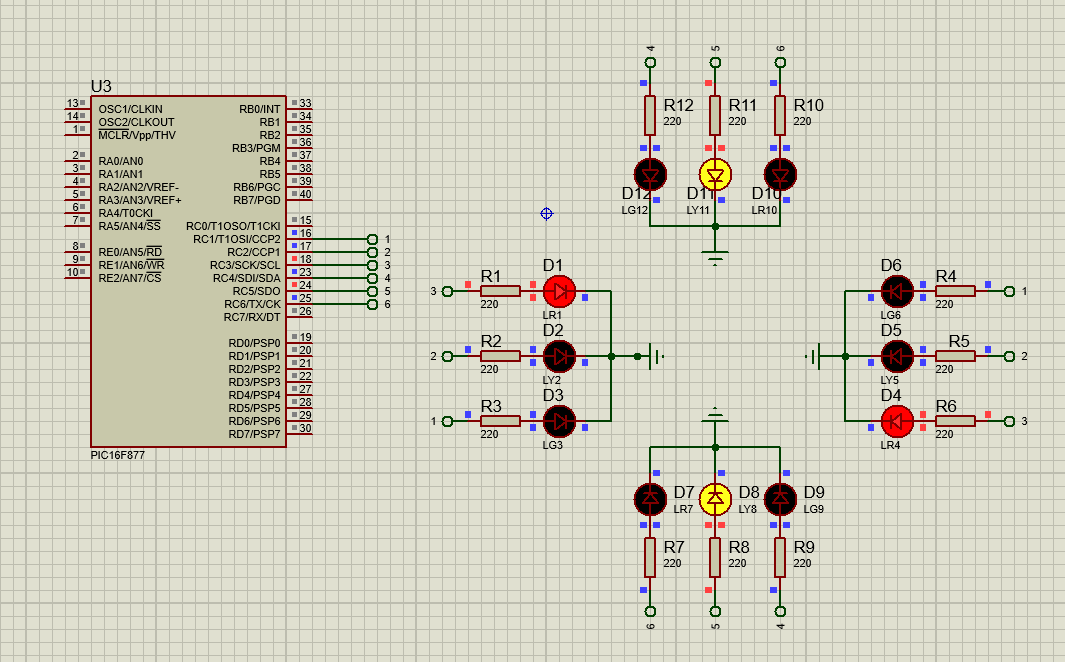
\includegraphics[width=5in]{source/picture/bai_1/lab1_ex3.2.png}
    \caption{\textit{Exercise 3 simulation: left-right yellow and up-down red}}
    \label{bai1_ex3_state_yellow_red}
\end{figure}

The demonstration video for this exercise is available at:
\begin{center}
    \url{https://github.com/quangnguyencomeng/CO3009-261-CC-2453052/blob/main/Lab/lab_reports/source/vids/lab1_ex3.mp4}
\end{center}

\textbf{Report 2: } The source code for the traffic-light controller is shown below. PORTC is used to control six LED outputs. The program repeatedly switches between the left-right direction and the up-down direction, with a yellow transition before each red phase.

\begin{lstlisting}[caption=Source code for Exercise 3]
#include <xc.h>
#define _XTAL_FREQ 4000000UL

#pragma config FOSC = XT
#pragma config WDTE = OFF
#pragma config PWRTE = ON
#pragma config BOREN = ON
#pragma config LVP = OFF
#pragma config CPD = OFF
#pragma config WRT = OFF
#pragma config CP = OFF

#define LR_GREEN   0x02  // RC1
#define LR_YELLOW  0x04  // RC2
#define LR_RED     0x08  // RC3

#define UD_GREEN   0x10  // RC4
#define UD_YELLOW  0x20  // RC5
#define UD_RED     0x40  // RC6

#define GREEN_TIME_MS   3000
#define YELLOW_TIME_MS  1000

void main(void)
{
    TRISC = 0x81;  // RC1-RC6 output, RC0 and RC7 input
    PORTC = 0x00;

    while (1)
    {
        PORTC = LR_GREEN | UD_RED;
        __delay_ms(GREEN_TIME_MS);

        PORTC = LR_YELLOW | UD_RED;
        __delay_ms(YELLOW_TIME_MS);

        PORTC = LR_RED | UD_GREEN;
        __delay_ms(GREEN_TIME_MS);

        PORTC = LR_RED | UD_YELLOW;
        __delay_ms(YELLOW_TIME_MS);
    }
}
\end{lstlisting}
\subsubsection{Exercise 4}
Add \textbf{only one 7 led segment} to the schematic in Exercise 3. This component can be found in Proteus by the keyword \textbf{7SEG-COM-ANODE}. For this device, the common pin should be connected to the power supply and other pins are supposed to connected to PB0 to PB6. Therefore, to turn-on a segment in this 7SEG, the STM32 pin should be in logic 0 (0V).\\

Implement a function named \textbf{display7SEG(int num)}. The input for this function is from 0 to 9 and the outputs are listed as following:

\begin{figure}[!htp]
    \centering
    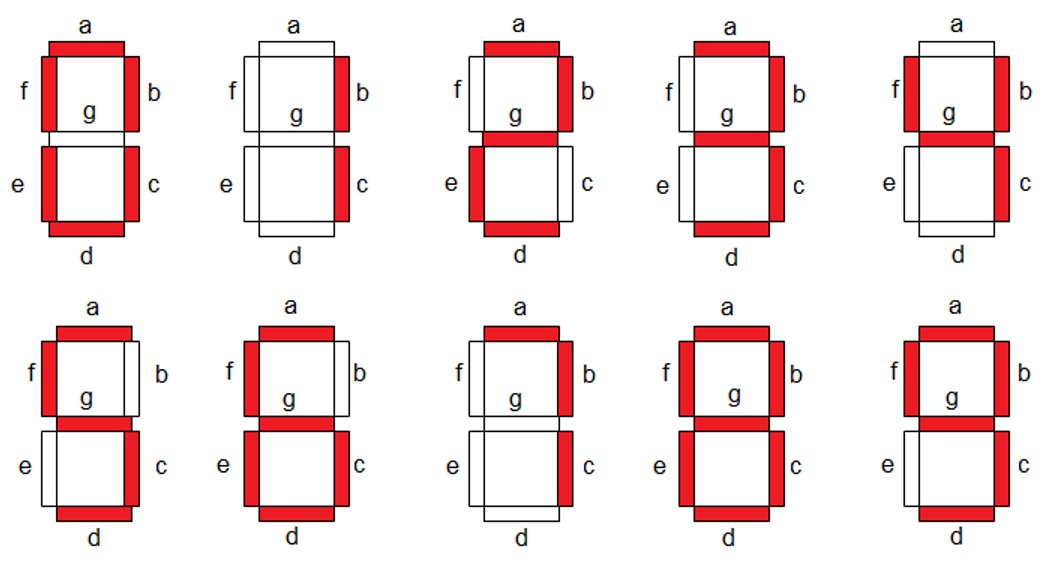
\includegraphics[width=4in]{source/picture/bai_1/pic3.PNG}
    \caption{\textit{Display a number on  7 segment LED}}
    \label{bai1_pic3}
\end{figure}

\newpage
This function is invoked in the while loop for testing as following:
\begin{lstlisting}[caption=An example for your source code]
int counter = 0;
while (1){
    if(counter >= 10) counter = 0;    
    display7SEG(counter++);
    HAL_Delay(1000);

}
\end{lstlisting}

\textbf{Report 1: } Figure \ref{bai1_ex4_schematic} shows the separate Proteus simulation. Its STM32F103C6 drives segments A--G through PA0--PA6, respectively. The display is common-anode, with the common pin connected to the supply; a GPIO output at logic 0 lights a segment. The submitted schematic uses PA0--PA6 rather than the PB0--PB6 suggested in the exercise description.

\begin{figure}[!htp]
    \centering
    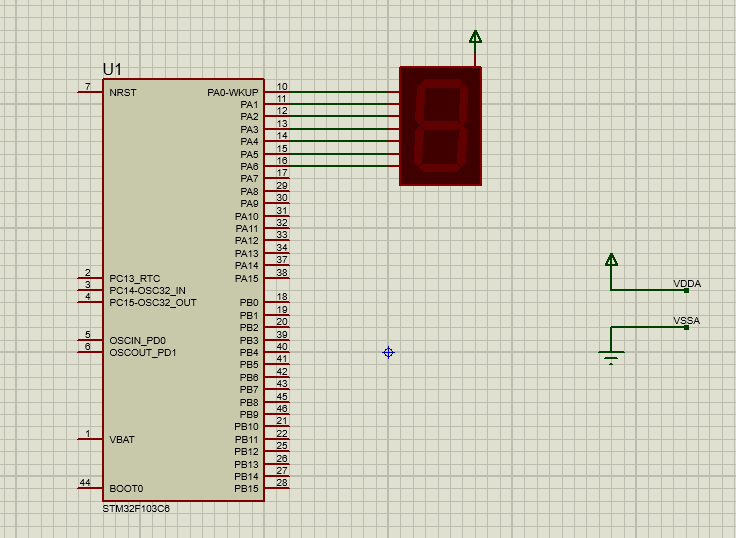
\includegraphics[width=5in]{source/picture/bai_1/lab_ex4.png}
    \caption{\textit{Proteus schematic for Exercise 4}}
    \label{bai1_ex4_schematic}
\end{figure}

The simulation video is available at:
\begin{center}
    \url{https://github.com/quangnguyencomeng/CO3009-261-CC-2453052/blob/main/Lab/lab_reports/source/vids/lab1_ex4.mp4}
\end{center}

\textbf{Report 2: } The source code of \texttt{PROTEUS\_LED\_BLINKY} matches the schematic: PA0--PA6 are connected to segments A--G. Since the display is common-anode, \texttt{GPIO\_PIN\_RESET} turns a segment on and \texttt{GPIO\_PIN\_SET} turns it off.

Instead of a hexadecimal pattern for each number, \texttt{setSegments} writes the value of each named GPIO pin. Each case of \texttt{display7SEG} then specifies the seven values in A--G order. The \texttt{SEGMENT\_PINS} mask is used only to initialize, test, or clear all segments.

\begin{lstlisting}[basicstyle=\ttfamily\small,caption={Pin-by-pin display7SEG implementation for the Proteus simulation}]
#define SEGMENT_PINS  (SEG_A_Pin | SEG_B_Pin | SEG_C_Pin | SEG_D_Pin | \
                       SEG_E_Pin | SEG_F_Pin | SEG_G_Pin)

/* Proteus common-anode display: RESET = on, SET = off. */
static void setSegments(GPIO_PinState a, GPIO_PinState b, GPIO_PinState c,
                        GPIO_PinState d, GPIO_PinState e, GPIO_PinState f,
                        GPIO_PinState g)
{
  HAL_GPIO_WritePin(SEG_A_GPIO_Port, SEG_A_Pin, a);
  HAL_GPIO_WritePin(SEG_B_GPIO_Port, SEG_B_Pin, b);
  HAL_GPIO_WritePin(SEG_C_GPIO_Port, SEG_C_Pin, c);
  HAL_GPIO_WritePin(SEG_D_GPIO_Port, SEG_D_Pin, d);
  HAL_GPIO_WritePin(SEG_E_GPIO_Port, SEG_E_Pin, e);
  HAL_GPIO_WritePin(SEG_F_GPIO_Port, SEG_F_Pin, f);
  HAL_GPIO_WritePin(SEG_G_GPIO_Port, SEG_G_Pin, g);
}

void display7SEG(int num)
{
  /* Each call lists the states of A, B, C, D, E, F and G in that order. */
  switch (num)
  {
    case 0:
      setSegments(GPIO_PIN_RESET, GPIO_PIN_RESET, GPIO_PIN_RESET, GPIO_PIN_RESET,
                  GPIO_PIN_RESET, GPIO_PIN_RESET, GPIO_PIN_SET);
      break;
    case 1:
      setSegments(GPIO_PIN_SET, GPIO_PIN_RESET, GPIO_PIN_RESET, GPIO_PIN_SET,
                  GPIO_PIN_SET, GPIO_PIN_SET, GPIO_PIN_SET);
      break;
    case 2:
      setSegments(GPIO_PIN_RESET, GPIO_PIN_RESET, GPIO_PIN_SET, GPIO_PIN_RESET,
                  GPIO_PIN_RESET, GPIO_PIN_SET, GPIO_PIN_RESET);
      break;
    case 3:
      setSegments(GPIO_PIN_RESET, GPIO_PIN_RESET, GPIO_PIN_RESET, GPIO_PIN_RESET,
                  GPIO_PIN_SET, GPIO_PIN_SET, GPIO_PIN_RESET);
      break;
    case 4:
      setSegments(GPIO_PIN_SET, GPIO_PIN_RESET, GPIO_PIN_RESET, GPIO_PIN_SET,
                  GPIO_PIN_SET, GPIO_PIN_RESET, GPIO_PIN_RESET);
      break;
    case 5:
      setSegments(GPIO_PIN_RESET, GPIO_PIN_SET, GPIO_PIN_RESET, GPIO_PIN_RESET,
                  GPIO_PIN_SET, GPIO_PIN_RESET, GPIO_PIN_RESET);
      break;
    case 6:
      setSegments(GPIO_PIN_RESET, GPIO_PIN_SET, GPIO_PIN_RESET, GPIO_PIN_RESET,
                  GPIO_PIN_RESET, GPIO_PIN_RESET, GPIO_PIN_RESET);
      break;
    case 7:
      setSegments(GPIO_PIN_RESET, GPIO_PIN_RESET, GPIO_PIN_RESET, GPIO_PIN_SET,
                  GPIO_PIN_SET, GPIO_PIN_SET, GPIO_PIN_SET);
      break;
    case 8:
      setSegments(GPIO_PIN_RESET, GPIO_PIN_RESET, GPIO_PIN_RESET, GPIO_PIN_RESET,
                  GPIO_PIN_RESET, GPIO_PIN_RESET, GPIO_PIN_RESET);
      break;
    case 9:
      setSegments(GPIO_PIN_RESET, GPIO_PIN_RESET, GPIO_PIN_RESET, GPIO_PIN_RESET,
                  GPIO_PIN_SET, GPIO_PIN_RESET, GPIO_PIN_RESET);
      break;
    default:
      HAL_GPIO_WritePin(GPIOA, SEGMENT_PINS, GPIO_PIN_SET);
      break;
  }
}
\end{lstlisting}

\subsubsection{Exercise 5}
Integrate the 7SEG-LED to the 4 way traffic light. In this case, the 7SEG-LED is used to display countdown value.\\

In this exercise, only source code is required to present. The function display7SEG in previous exercise can be re-used.

\textbf{Report: } Figure \ref{bai1_ex5_schematic} shows the Proteus circuit with four traffic-light poles and two common-anode 7-segment displays. Poles 1 and 2 form one opposite pair and share display 1; poles 3 and 4 form the other pair and share display 2. Segments A--G of display 1 use PA0--PA6, and those of display 2 use PA7--PA13. The twelve traffic LEDs use PB0--PB11, with green, yellow and red assigned in that order for each pole. In the final wiring, PB10 drives the yellow LED of pole 4 and PB11 drives its red LED.

\begin{figure}[!htp]
    \centering
    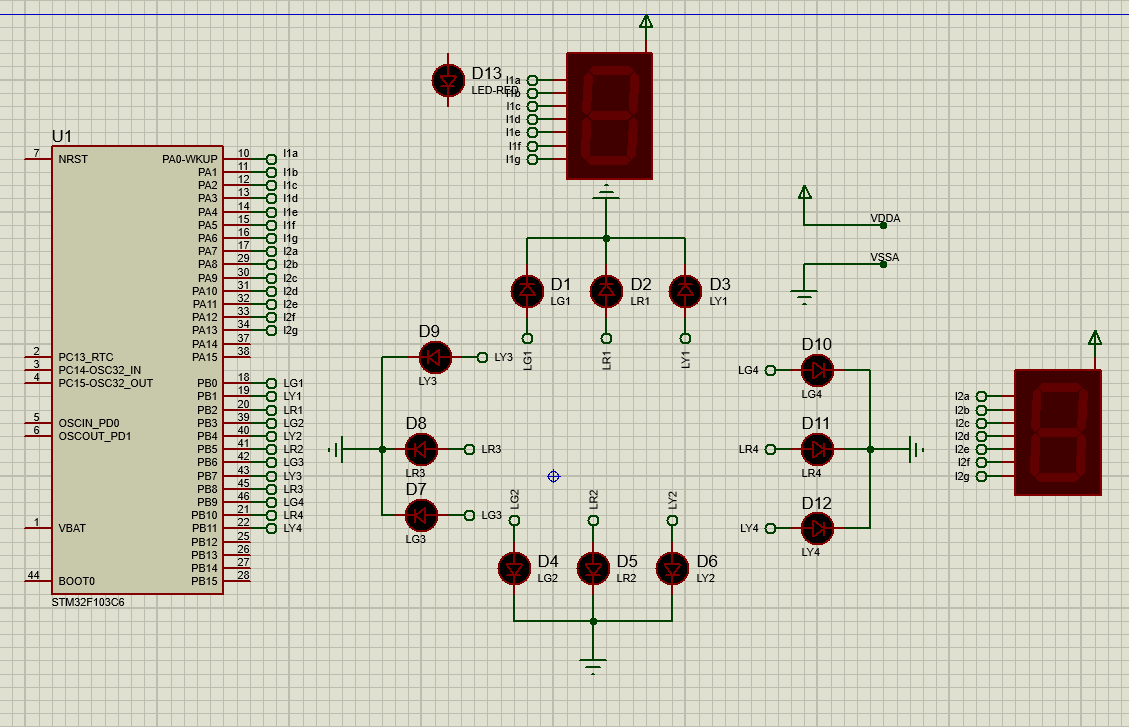
\includegraphics[width=5.5in]{source/picture/bai_1/lab1_ex5.png}
    \caption{\textit{Proteus schematic for Exercise 5}}
    \label{bai1_ex5_schematic}
\end{figure}

The simulation video is available at:
\begin{center}
    \url{https://github.com/quangnguyencomeng/CO3009-261-CC-2453052/blob/main/Lab/lab_reports/source/vids/lab1_ex5.mp4}
\end{center}

One complete cycle lasts 10 seconds. While poles 1--2 are green for 3 seconds and yellow for 2 seconds, poles 3--4 remain red for 5 seconds. The two pairs then exchange roles. Each display shows the remaining seconds for its own pair: 3--2--1 during green, 2--1 during yellow, and 5--4--3--2--1 during red.

The code extends the Exercise 4 digit function to \texttt{display7SEG(display, num)}. The first argument chooses one of the two displays; the digit cases still set segments A--G individually, without hexadecimal digit patterns. Since both displays are common-anode, \texttt{GPIO\_PIN\_RESET} lights a segment. The traffic LEDs have their cathodes connected to ground, so \texttt{GPIO\_PIN\_SET} lights an LED. The following source excerpts show the pin-by-pin output functions and the traffic-light cycle.

\begin{lstlisting}[basicstyle=\ttfamily\small,caption={Exercise 5: selecting a display and controlling each traffic LED}]
/* Common-anode 7-segment displays: RESET = on. */
static void setSegments(uint8_t display, GPIO_PinState a, GPIO_PinState b,
                        GPIO_PinState c, GPIO_PinState d, GPIO_PinState e,
                        GPIO_PinState f, GPIO_PinState g)
{
  uint16_t pinA = (display == 1U) ? SEG1_A_Pin : SEG2_A_Pin;
  uint16_t pinB = (display == 1U) ? SEG1_B_Pin : SEG2_B_Pin;
  uint16_t pinC = (display == 1U) ? SEG1_C_Pin : SEG2_C_Pin;
  uint16_t pinD = (display == 1U) ? SEG1_D_Pin : SEG2_D_Pin;
  uint16_t pinE = (display == 1U) ? SEG1_E_Pin : SEG2_E_Pin;
  uint16_t pinF = (display == 1U) ? SEG1_F_Pin : SEG2_F_Pin;
  uint16_t pinG = (display == 1U) ? SEG1_G_Pin : SEG2_G_Pin;

  HAL_GPIO_WritePin(GPIOA, pinA, a);
  HAL_GPIO_WritePin(GPIOA, pinB, b);
  HAL_GPIO_WritePin(GPIOA, pinC, c);
  HAL_GPIO_WritePin(GPIOA, pinD, d);
  HAL_GPIO_WritePin(GPIOA, pinE, e);
  HAL_GPIO_WritePin(GPIOA, pinF, f);
  HAL_GPIO_WritePin(GPIOA, pinG, g);
}

/* Traffic LEDs: SET = on. Arguments are G, Y, R for poles 1--4. */
static void setTraffic(GPIO_PinState lg1, GPIO_PinState ly1,
                       GPIO_PinState lr1, GPIO_PinState lg2,
                       GPIO_PinState ly2, GPIO_PinState lr2,
                       GPIO_PinState lg3, GPIO_PinState ly3,
                       GPIO_PinState lr3, GPIO_PinState lg4,
                       GPIO_PinState ly4, GPIO_PinState lr4)
{
  HAL_GPIO_WritePin(GPIOB, LG1_Pin, lg1);
  HAL_GPIO_WritePin(GPIOB, LY1_Pin, ly1);
  HAL_GPIO_WritePin(GPIOB, LR1_Pin, lr1);
  HAL_GPIO_WritePin(GPIOB, LG2_Pin, lg2);
  HAL_GPIO_WritePin(GPIOB, LY2_Pin, ly2);
  HAL_GPIO_WritePin(GPIOB, LR2_Pin, lr2);
  HAL_GPIO_WritePin(GPIOB, LG3_Pin, lg3);
  HAL_GPIO_WritePin(GPIOB, LY3_Pin, ly3);
  HAL_GPIO_WritePin(GPIOB, LR3_Pin, lr3);
  HAL_GPIO_WritePin(GPIOB, LG4_Pin, lg4);
  HAL_GPIO_WritePin(GPIOB, LY4_Pin, ly4);
  HAL_GPIO_WritePin(GPIOB, LR4_Pin, lr4);
}
\end{lstlisting}

\begin{lstlisting}[basicstyle=\ttfamily\small,caption={Exercise 5: countdown and traffic-light sequence}]
/* In the main loop; display7SEG is the pin-by-pin function
   from Exercise 4, extended with a display selector. */
while (1)
{
  /* Poles 1--2: green 3 s, yellow 2 s.
     Poles 3--4: red 5 s. */
  for (int t = 5; t > 0; --t)
  {
    if (t > 2)
    {
      setTraffic(GPIO_PIN_SET,   GPIO_PIN_RESET, GPIO_PIN_RESET,
                 GPIO_PIN_SET,   GPIO_PIN_RESET, GPIO_PIN_RESET,
                 GPIO_PIN_RESET, GPIO_PIN_RESET, GPIO_PIN_SET,
                 GPIO_PIN_RESET, GPIO_PIN_RESET, GPIO_PIN_SET);
      display7SEG(1, t - 2);
    }
    else
    {
      setTraffic(GPIO_PIN_RESET, GPIO_PIN_SET,   GPIO_PIN_RESET,
                 GPIO_PIN_RESET, GPIO_PIN_SET,   GPIO_PIN_RESET,
                 GPIO_PIN_RESET, GPIO_PIN_RESET, GPIO_PIN_SET,
                 GPIO_PIN_RESET, GPIO_PIN_RESET, GPIO_PIN_SET);
      display7SEG(1, t);
    }
    display7SEG(2, t);
    HAL_Delay(1000);
  }

  /* Poles 1--2: red 5 s.
     Poles 3--4: green 3 s, yellow 2 s. */
  for (int t = 5; t > 0; --t)
  {
    display7SEG(1, t);
    if (t > 2)
    {
      setTraffic(GPIO_PIN_RESET, GPIO_PIN_RESET, GPIO_PIN_SET,
                 GPIO_PIN_RESET, GPIO_PIN_RESET, GPIO_PIN_SET,
                 GPIO_PIN_SET,   GPIO_PIN_RESET, GPIO_PIN_RESET,
                 GPIO_PIN_SET,   GPIO_PIN_RESET, GPIO_PIN_RESET);
      display7SEG(2, t - 2);
    }
    else
    {
      setTraffic(GPIO_PIN_RESET, GPIO_PIN_RESET, GPIO_PIN_SET,
                 GPIO_PIN_RESET, GPIO_PIN_RESET, GPIO_PIN_SET,
                 GPIO_PIN_RESET, GPIO_PIN_SET,   GPIO_PIN_RESET,
                 GPIO_PIN_RESET, GPIO_PIN_SET,   GPIO_PIN_RESET);
      display7SEG(2, t);
    }
    HAL_Delay(1000);
  }
}
\end{lstlisting}

\subsubsection{Exercise 6}
In this exercise, a new Proteus schematic is designed to simulate an analog clock, with 12 different number. The connections for 12 LEDs are supposed from PA4 to PA15 of the STM32. The arrangement of 12 LEDs is depicted as follows.

\begin{figure}[!htp]
    \centering
    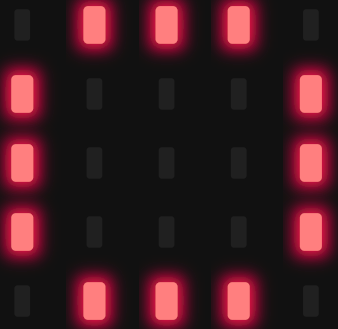
\includegraphics[width=3in]{source/picture/bai_1/pic4.PNG}
    \caption{\textit{12 LEDs for an analog clock}}
    \label{bai1_ex6_layout}
\end{figure}

Report 1: Present the schematic.
Report 2: Implement a simple program to test the connection of every single LED. This testing program should turn every LED in a sequence.

\textbf{Report 1: } Figure \ref{bai1_ex6_schematic} presents the Proteus schematic built for this exercise. The twelve LEDs are arranged as a clock face and numbered 0--11, as in Figure \ref{bai1_ex6_layout}. LED 0 is connected to PA4, LED 1 to PA5, and so on through LED 11 on PA15. Their cathodes are connected to ground, so a high GPIO output turns the selected LED on. All twelve pins are configured as push-pull GPIO outputs in the \texttt{IDE\_ANA\_CLOCK} project; the debug interface is disabled in the IOC configuration so PA13--PA15 can be used as outputs.

\begin{figure}[!htp]
    \centering
    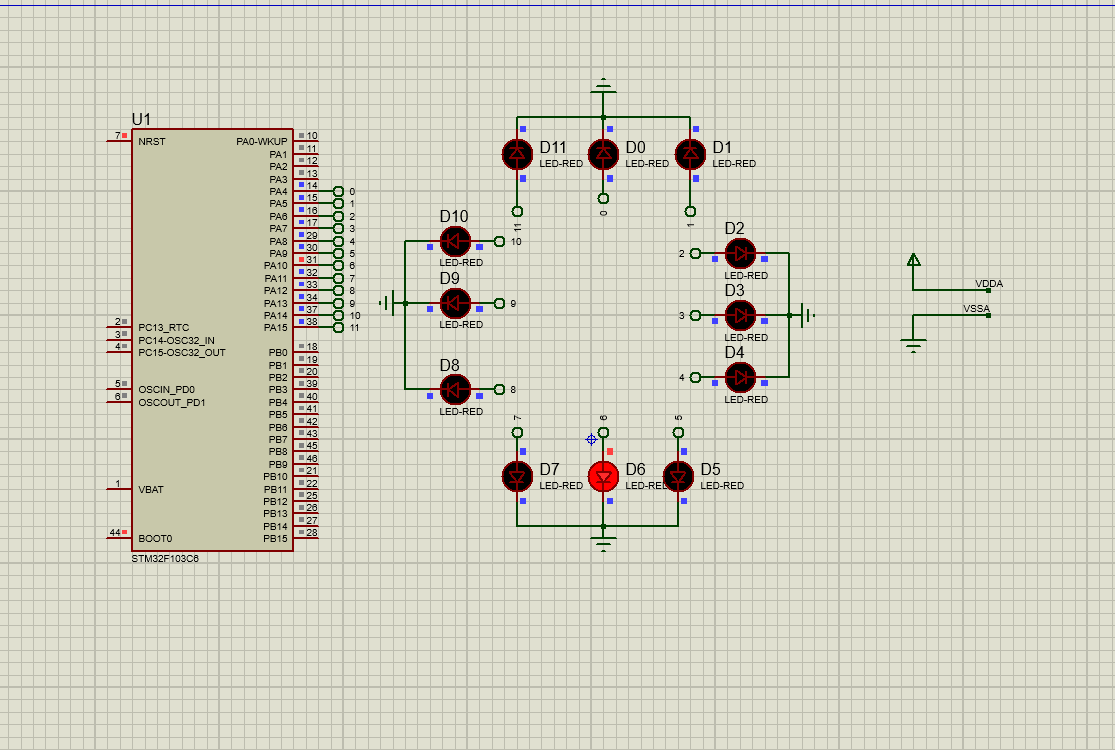
\includegraphics[width=5.5in]{source/picture/bai_1/lab1_ex6.png}
    \caption{\textit{Proteus schematic of the 12-LED analog-clock test}}
    \label{bai1_ex6_schematic}
\end{figure}

The simulation video is available at:
\begin{center}
    \url{https://github.com/quangnguyencomeng/CO3009-261-CC-2453052/blob/main/Lab/lab_reports/source/vids/lab1_ex6.mp4}
\end{center}

\textbf{Report 2: } The following excerpts from \texttt{IDE\_ANA\_CLOCK/Core/Src/main.c} implement the connection test. The program first clears the clock face, then lights each LED in numerical order for 300 ms and switches it off before moving to the next one. Thus, only one LED is intended to be on at a time. For example, number 0 selects PA4 and number 11 selects PA15.

\begin{lstlisting}[basicstyle=\ttfamily\small,caption={Exercise 6: GPIO initialization and sequential test of the 12 clock LEDs}]
#define CLOCK_ALL_PINS (GPIO_PIN_4 | GPIO_PIN_5 | GPIO_PIN_6 | GPIO_PIN_7 | \
                        GPIO_PIN_8 | GPIO_PIN_9 | GPIO_PIN_10 | GPIO_PIN_11 | \
                        GPIO_PIN_12 | GPIO_PIN_13 | GPIO_PIN_14 | GPIO_PIN_15)

void clearAllClock(void)
{
  HAL_GPIO_WritePin(GPIOA, CLOCK_ALL_PINS, GPIO_PIN_RESET);
}

void setNumberOnClock(int num)
{
  if (num >= 0 && num < 12)
  {
    uint16_t pin = (uint16_t)(GPIO_PIN_4 << num);
    HAL_GPIO_WritePin(GPIOA, pin, GPIO_PIN_SET);
  }
}

void clearNumberOnClock(int num)
{
  if (num >= 0 && num < 12)
  {
    uint16_t pin = (uint16_t)(GPIO_PIN_4 << num);
    HAL_GPIO_WritePin(GPIOA, pin, GPIO_PIN_RESET);
  }
}

static void MX_GPIO_Init(void)
{
  GPIO_InitTypeDef GPIO_InitStruct = {0};
  __HAL_RCC_GPIOA_CLK_ENABLE();
  HAL_GPIO_WritePin(GPIOA, CLOCK_ALL_PINS, GPIO_PIN_RESET);
  GPIO_InitStruct.Pin = CLOCK_ALL_PINS;
  GPIO_InitStruct.Mode = GPIO_MODE_OUTPUT_PP;
  GPIO_InitStruct.Pull = GPIO_NOPULL;
  GPIO_InitStruct.Speed = GPIO_SPEED_FREQ_LOW;
  HAL_GPIO_Init(GPIOA, &GPIO_InitStruct);
}

int main(void)
{
  HAL_Init();
  SystemClock_Config();
  MX_GPIO_Init();
  clearAllClock();
  while (1)
  {
    for (int num = 0; num < 12; ++num)
    {
      setNumberOnClock(num);
      HAL_Delay(300);
      clearNumberOnClock(num);
    }
  }
}
\end{lstlisting}

\subsubsection{Exercise 7}
Implement a function named \textbf{clearAllClock()} to turn off all 12 LEDs. Present the source code of this function.

\textbf{Report: } All twelve LEDs in the clock schematic have their cathodes connected to ground. Therefore, writing \texttt{GPIO\_PIN\_RESET} to PA4--PA15 turns them all off. \texttt{CLOCK\_ALL\_PINS} is the mask of these twelve pins, defined in Exercise 6. The function in \texttt{IDE\_ANA\_CLOCK/Core/Src/main.c} is:

\begin{lstlisting}[caption={Exercise 7: turn off all 12 clock LEDs}]
void clearAllClock(void)
{
  HAL_GPIO_WritePin(GPIOA, CLOCK_ALL_PINS, GPIO_PIN_RESET);
}
\end{lstlisting}

\subsubsection{Exercise 8}
Implement a function named \textbf{setNumberOnClock(int num)}. The input for this function is from \textbf{0 to 11} and an appropriate LED is turn on. Present the source code of this function.

\textbf{Report: } LED 0 (the 12 o'clock position) is connected to PA4; LED 1 is connected to PA5, continuing in order to LED 11 on PA15. After checking that \texttt{num} is within 0--11, the function shifts the PA4 pin mask by \texttt{num} places and sets that GPIO output HIGH. The corresponding LED then turns on.

\begin{lstlisting}[caption={Exercise 8: turn on the LED selected by num}]
void setNumberOnClock(int num)
{
  if (num >= 0 && num < 12)
  {
    uint16_t pin = (uint16_t)(GPIO_PIN_4 << num);
    HAL_GPIO_WritePin(GPIOA, pin, GPIO_PIN_SET);
  }
}
\end{lstlisting}

Figure \ref{bai1_ex8_simulation} shows the Proteus simulation. The test loop used for Exercise 8 in \texttt{IDE\_ANA\_CLOCK/Core/Src/main.c} waits three seconds and calls \texttt{setNumberOnClock(10)}, which selects PA14. Since this test does not clear that LED afterward, it remains lit.

\begin{figure}[!htp]
    \centering
    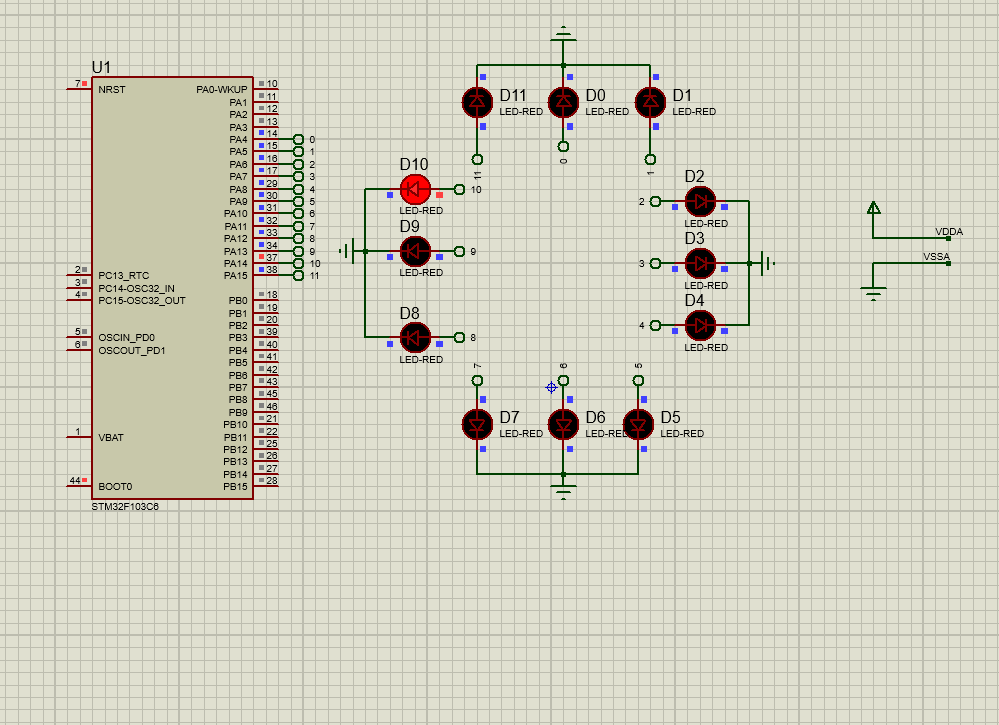
\includegraphics[width=5.5in]{source/picture/bai_1/lab1_ex8.png}
    \caption{\textit{Proteus simulation for Exercise 8}}
    \label{bai1_ex8_simulation}
\end{figure}

\begin{lstlisting}[caption={Exercise 8: test call in the main loop}]
clearAllClock();
while (1)
{
  HAL_Delay(3000);
  setNumberOnClock(10);
}
\end{lstlisting}

The simulation video is available at:
\begin{center}
    \url{https://github.com/quangnguyencomeng/CO3009-261-CC-2453052/blob/main/Lab/lab_reports/source/vids/lab1_ex8.mp4}
\end{center}

\subsubsection{Exercise 9}
Implement a function named \textbf{clearNumberOnClock(int num)}. The input for this function is from \textbf{0 to 11} and the corresponding LED is turned off.

\textbf{Report: } As in Exercise 8, LED 0 is connected to PA4 and LED 11 to PA15. The function checks that \texttt{num} is within 0--11, shifts the PA4 mask to select that LED, and writes \texttt{GPIO\_PIN\_RESET}. Since the LEDs are active-high, this turns off only the selected LED.

\begin{lstlisting}[caption={Exercise 9: turn off the LED selected by num}]
void clearNumberOnClock(int num)
{
  if (num >= 0 && num < 12)
  {
    uint16_t pin = (uint16_t)(GPIO_PIN_4 << num);
    HAL_GPIO_WritePin(GPIOA, pin, GPIO_PIN_RESET);
  }
}
\end{lstlisting}

To test the function, the program first turns on all twelve LEDs. After three seconds, it calls \texttt{clearNumberOnClock(10)}. Number 10 corresponds to PA14, so that LED turns off while the others remain on. The relevant code supplied for this exercise is:

\begin{lstlisting}[caption={Exercise 9: turn on all LEDs, then clear number 10}]
void lightAllClock(void)
{
  HAL_GPIO_WritePin(GPIOA, CLOCK_ALL_PINS, GPIO_PIN_SET);
}

clearAllClock();
int turn_on_all_leds = 0;
while (1)
{
  if (!turn_on_all_leds)
  {
    lightAllClock();
    HAL_Delay(3000);
    turn_on_all_leds++;
  }
  clearNumberOnClock(10);
}
\end{lstlisting}

\begin{figure}[!htp]
    \centering
    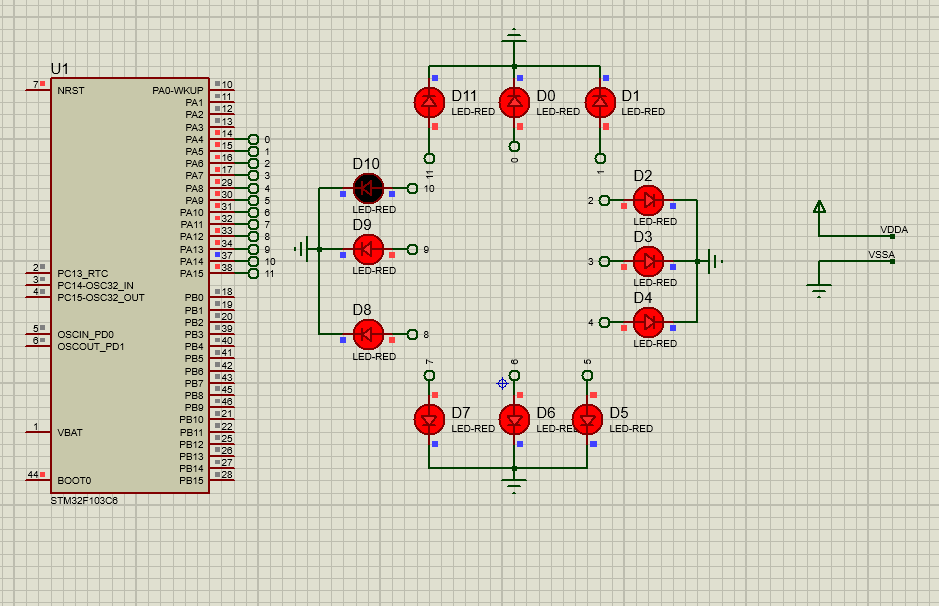
\includegraphics[width=5.5in]{source/picture/bai_1/lab1_ex9.png}
    \caption{\textit{Proteus simulation after turning off LED 10 in Exercise 9}}
    \label{bai1_ex9_simulation}
\end{figure}

The simulation video is available at:
\begin{center}
    \url{https://github.com/quangnguyencomeng/CO3009-261-CC-2453052/blob/main/Lab/lab_reports/source/vids/lab1_ex9.mp4}
\end{center}

\subsubsection{Exercise 10}
Integrate the whole system and use 12 LEDs to display a clock. At a given time, there are only 3 LEDs are turn on for hour, minute and second information.

\textbf{Report: } The program starts at 10:10:00 for the simulation. LED 0 is the 12 o'clock position. The hour hand selects \texttt{hour \% 12}; the minute and second hands select \texttt{minute / 5} and \texttt{second / 5}, respectively, because each of the twelve positions represents five minutes or five seconds. Every second, the program clears the previous positions, lights the three selected positions, and advances the time. At 60 seconds it increments the minute; at 60 minutes it increments the hour; after 12 o'clock it returns to 1 o'clock. The initial values can be changed in \texttt{main.c}.

When two hands point to the same position, they share one physical LED, so fewer than three separate LEDs are visible at that instant. The circuit has one LED per position and cannot distinguish overlapping hands.

\begin{lstlisting}[basicstyle=\ttfamily\small,caption={Exercise 10: software clock using the twelve LEDs}]
/* In main(), before HAL_Init(): */
int hour = 10;
int minute = 10;
int second = 0;

/* After HAL_Init(), SystemClock_Config() and MX_GPIO_Init(): */
clearAllClock();
while (1)
{
  clearAllClock();
  setNumberOnClock(hour % 12);
  setNumberOnClock(minute / 5);
  setNumberOnClock(second / 5);

  HAL_Delay(1000);
  second++;
  if (second == 60)
  {
    second = 0;
    minute++;
    if (minute == 60)
    {
      minute = 0;
      hour++;
      if (hour == 13)
      {
        hour = 1;
      }
    }
  }
}
\end{lstlisting}

Figure \ref{bai1_ex10_simulation} shows a captured state with the hour, minute, and second LEDs at positions 10, 2, and 4. Figure \ref{bai1_ex10_five_minutes} shows a later state: the minute LED has advanced to position 3, while the hour and second LEDs are at positions 10 and 7.

\begin{figure}[!htp]
    \centering
    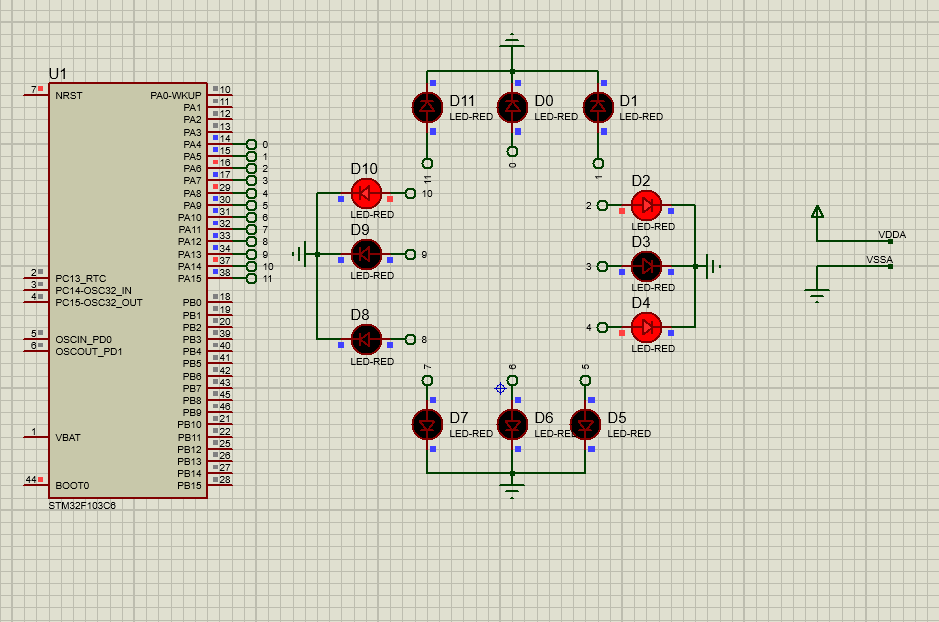
\includegraphics[width=5.5in]{source/picture/bai_1/lab1_ex10.png}
    \caption{\textit{Proteus simulation of the twelve-LED clock in Exercise 10}}
    \label{bai1_ex10_simulation}
\end{figure}

\begin{figure}[!htp]
    \centering
    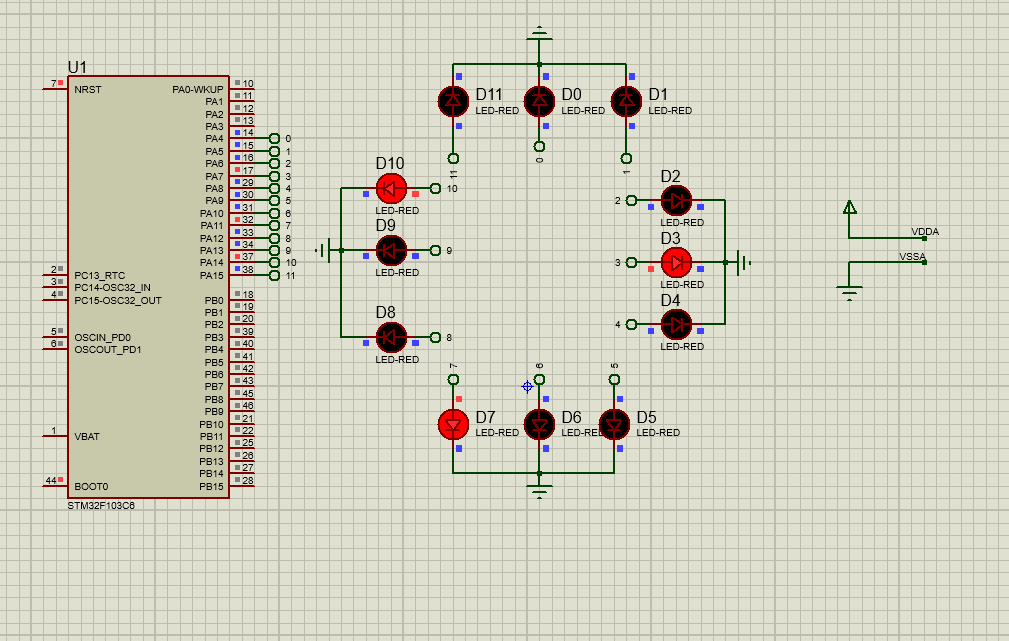
\includegraphics[width=5.5in]{source/picture/bai_1/lab1_ex10_5min.png}
    \caption{\textit{Proteus simulation after the minute LED advances in Exercise 10}}
    \label{bai1_ex10_five_minutes}
\end{figure}

The two simulation recordings are available at:
\begin{center}
    \url{https://github.com/quangnguyencomeng/CO3009-261-CC-2453052/blob/main/Lab/lab_reports/source/vids/lab1_ex10.mp4}\\
    \url{https://github.com/quangnguyencomeng/CO3009-261-CC-2453052/blob/main/Lab/lab_reports/source/vids/lab1_ex10_5min.mp4}
\end{center}
